\documentclass{article}
\usepackage[utf8]{inputenc}
\usepackage[english]{babel}
\usepackage[font=small,labelfont=bf]{caption}
\usepackage{geometry}
\usepackage{natbib}
\usepackage{pxfonts}
\usepackage{graphicx}
\usepackage{newfloat}
\usepackage{setspace}
\usepackage{hyperref}
\usepackage{lineno}
\usepackage{placeins}

\newcommand{\argmax}{\mathop{\mathrm{argmax}}\limits}

\newcommand{\topicopt}{S1}
\newcommand{\topics}{S2}
\newcommand{\featureimportance}{S3}
\newcommand{\corrmats}{S4}
\newcommand{\matchmats}{S5}
\newcommand{\kopt}{S6}

\doublespacing
\linenumbers

\title{Geometric models reveal behavioral and neural signatures of how naturalistic experiences are transformed into episodic memories}
  
\author{Andrew C. Heusser\textsuperscript{1, 2, \textdagger}, Paxton C. Fitzpatrick\textsuperscript{1, \textdagger}, and Jeremy R. Manning\textsuperscript{1, *}\\\textsuperscript{1}Department of Psychological and Brain Sciences\\Dartmouth College, Hanover, NH 03755, USA\\\textsuperscript{2}Akili Interactive\\Boston, MA 02110\\\textsuperscript{\textdagger}Denotes equal contribution\\\textsuperscript{*}Corresponding author: Jeremy.R.Manning@Dartmouth.edu}

\bibliographystyle{apa}

\begin{document}
\maketitle

\begin{abstract}
Our ongoing subjective experience reflects external sensory information from each moment, along with additional information from our past that we carry with us into that moment.  The blend of memories, knowledge, emotions, goals, and other internal perceptual and mental states that color our subjective experience provides a \textit{context} for interpreting new information and conceptually linking what is happening now with our prior experiences.  Because this contextual information is often person-specific, the subjective experience that each person encodes into their memory is often idiosyncratic, even for shared experiences and sensory perspectives.  We sought to study which aspects of a shared naturalistic experience were preserved or distorted, and how those distortions compared across individuals.  To this end, we developed a geometric framework for mathematically characterizing the subjective conceptual content of dynamic naturalistic experiences.  We model experiences as \textit{trajectories} through word embedding spaces whose coordinates reflect the universe of thoughts under consideration.  We also demonstrate how \textit{memories} may also be modeled as trajectories through the same spaces.  According to this view, encoding an experience into memory entails geometrically distorting or transforming the \textit{shape} of the original experience's trajectory.  This translates qualitative, neuropsychological questions about how we remember naturalistic experiences into quantitive, geometric questions about the spatial configurations of trajectory shapes.  We applied our framework to data collected as participants watched and verbally recounted a television episode while undergoing functional neuroimaging.  We found that the trajectories of participants' recountings of the episode nearly all captured the coarse spatial properties of the original episode's trajectory (i.e., the essential plot points), but participants differed in their memory for fine details.  We also identified a network of brain structures that were sensitive to the shape of the episode's trajectory through word embedding space, and an overlapping network that predicted, at the time of encoding, how people would distort (transform) the episode's trajectory when they recounted the episode later.  Our work provides insights into how our brains distort and transform our ongoing experiences when we encode them into episodic memories.
\end{abstract}


\section*{Introduction}
What does it mean to \textit{remember} something? In traditional episodic memory experiments \citep[e.g., list-learning or trial-based experiments;][]{Murd62a, Kaha96}, remembering is often cast as a discrete and binary operation: each studied item may be separated from the rest of one's experience and singularly labeled as having been recalled or forgotten. More nuanced studies might incorporate self-reported confidence measures as a proxy for memory strength, or ask participants to discriminate between ``recollecting'' the (contextual) details of an experience or having a general feeling of ``familiarity'' \citep{Yone02}. Using well-controlled, trial-based experimental designs, the field has amassed a wealth of information regarding human episodic memory.  However, there are fundamental properties of the external world and our memories that trial-based experiments are not well suited to capture~\citep[for review, also see][]{KoriGold94, HukEtal18}.  First, our experiences and memories are continuous, rather than discrete---isolating a (naturalistic) event from the context in which it occurs can substantially change its meaning.  Second, whether or not the rememberer has precisely reproduced a specific set of words in describing a given experience is nearly orthogonal to how well they were actually able to remember it.  In classic (e.g., list-learning) memory studies, by contrast, the number or proportion of \textit{exact} recalls is often considered to be a primary metric for assessing the quality of participants' memories.  Third, one might remember the \textit{essence} (or a general summary) of an experience but forget (or neglect to recount) particular details.  Capturing the essence of what happened is often a main goal of recounting an episodic memory to a listener, whereas the inclusion of specific, low-level details is often less pertinent.

How might we formally characterize the \textit{essence} of an experience, and whether it has been recovered by the rememberer?  And how might we distinguish an experience's overarching essence from its low-level details?  One approach is to start by considering some fundamental properties of the dynamics of our experiences.  Each given moment of an experience tends to derive meaning from surrounding moments, as well as from longer-range temporal associations~\citep{LernEtal11, Mann19, Mann20}.  Therefore, the timecourse describing how an event unfolds is fundamental to its overall meaning.  Further, this hierarchy formed by our subjective experiences at different timescales defines a \textit{context} for each new moment~\citep[e.g.,][]{HowaKaha02a, HowaEtal14}, and plays an important role in how we interpret that moment and remember it later~\citep[for review see][]{MannEtal15, Mann20}.  Our memory systems can leverage these associations to form predictions that help guide our behaviors~\citep{RangRitc12}.  For example, as we navigate the world, the features of our subjective experiences tend to change gradually (e.g., the room or situation we find ourselves in at any given moment is strongly temporally autocorrelated), allowing us to form stable estimates of our current situation and behave accordingly~\citep{ZackEtal07, ZwaaRadv98}.

Occasionally, this gradual ``drift" of our ongoing experience is punctuated by sudden changes, or ``shifts"~\citep[e.g., when we walk through a doorway; ][]{RadvZack17}.  Prior research suggests that these sharp transitions (termed \textit{event boundaries}) help to discretize our experiences (and their mental representations) into \textit{events}~\citep{RadvZack17, BrunEtal18, HeusEtal18b, ClewDava17, EzzyDava11, DuBrDava13}.  The interplay between the stable (within-event) and transient (across-event) temporal dynamics of an experience also provides a potential framework for transforming experiences into memories that distills those experiences down to their essence.  For example, prior work has shown that event boundaries can influence how we learn sequences of items~\citep{HeusEtal18b, DuBrDava13}, navigate~\citep{BrunEtal18}, and remember and understand narratives~\citep{ZwaaRadv98, EzzyDava11}.  This work also suggests a means of distinguishing the essence of an experience from its low-level details.  The overall structure of events and event transitions reflects how the high-level experience unfolds (i.e., its essence), while subtler event-level properties reflect low-level details.  Prior research has also implicated a network of brain regions (including the hippocampus and the medial prefrontal cortex) in playing a critical role in transforming experiences into structured and consolidated memories ~\citep{TompDava17}.

Here, we sought to examine how the temporal dynamics of a ``naturalistic'' experience were later reflected in participants' memories.  We also sought to leverage the above conceptual insights into the distinctions between an experience's essence and low-level details to build models that explicitly quantified these distinctions.  We analyzed an open dataset that comprised behavioral and functional Magnetic Resonance Imaging (fMRI) data collected as participants viewed and then verbally recounted an episode of the BBC television series \textit{Sherlock}~\citep{ChenEtal17}.  We developed a computational framework for characterizing the temporal dynamics of the moment-by-moment content of the episode, and of participants' verbal recalls.  Specifically, we use topic modeling~\citep{BleiEtal03} to characterize the thematic conceptual (semantic) content present in each moment of the episode and recalls, and hidden Markov models~\citep{Rabi89, BaldEtal17} to discretize this evolving semantic content into events.  In this way, we cast both naturalistic experiences and memories of those experiences as geometric \textit{trajectories} that describe how they evolve over time. Under this framework, successful remembering entails verbally ``traversing'' the content trajectory of the episode, thereby reproducing the shape (essence) of the original experience.  Our framework captures the episode's essence in the sequence of geometric coordinates for its events, and its low-level details by examining its within-event geometric properties.

Comparing the overall shapes of the topic trajectories for the episode and participants' recalls reveals which aspects of the episode's essence were preserved (or discarded) in the translation into memory.  We also develop two metrics for assessing participants' memories for low-level details: (1) the \textit{precision} with which a participant recounts details about each event, and (2) the \textit{distinctiveness} of each recall event, relative to other recalled events.  We examine how these metrics relate to overall memory performance as judged by third-party human annotators.  We also compare and contrast our general approach to studying memory for naturalistic experiences with standard metrics for assessing performance on more traditional memory tasks, such as list-learning.  Last, we leverage our framework to identify networks of brain structures whose responses (as participants watched the episode) reflected the temporal dynamics of either the episode or how participants would later recount it.


\section*{Results}
To characterize the dynamic content of the \textit{Sherlock} episode and participants' subsequent recountings, we used a topic model~\citep{BleiEtal03} to discover the episode's latent themes.  Topic models take as inputs a vocabulary of words to consider and a collection of text documents, and return two output matrices.  The first of these is a \textit{topics matrix} whose rows are \textit{topics} (or latent themes) and whose columns correspond to words in the vocabulary. The entries in the topics matrix reflect how each word in the vocabulary is weighted by each discovered topic.  For example, a detective-themed topic might weight heavily on words like ``crime,'' and ``search.''  The second output is a \textit{topic proportions matrix}, with one row per document and one column per topic.  The topic proportions matrix describes the mixture of discovered topics reflected in each document.

\cite{ChenEtal17} collected hand-annotated information about each of 1,000 (manually identified) scenes spanning the roughly 50 minute video used in their experiment.  This information included: a brief narrative description of what was happening, the location where the scene took place, the names of any characters on the screen, and other similar details (for a full list of annotated features, see \textit{Methods}).  We took from these annotations the union of all unique words (excluding stop words, such as ``and,'' ``or,'' ``but,'' etc.) across all features and scenes as the ``vocabulary'' for the topic model.  We then concatenated the sets of words across all features contained in overlapping sliding windows of (up to) 50 scenes, and treated each window as a single ``document" for the purpose of fitting the topic model.  Next, we fit a topic model with (up to) $K = 100$ topics to this collection of documents.  We found that 32 unique topics (with non-zero weights) were sufficient to describe the time-varying content of the episode (see \textit{Methods}; Figs.~\ref{fig:schematic}, \topics).  Note that our approach is similar in some respects to Dynamic Topic Models~\citep{BleiLaff06}, in that we sought to characterize how the thematic content of the episode evolved over time.  However, whereas Dynamic Topic Models are designed to characterize how the properties of \textit{collections} of documents change over time, our sliding window approach allows us to examine the topic dynamics within a single document (or video).  Specifically, our approach yielded (via the topic proportions matrix) a single \textit{topic vector} for each sliding window of annotations transformed by the topic model.  We then stretched (interpolated) the resulting windows-by-topics matrix to match the time series of the 1,976 fMRI volumes collected as participants viewed the episode.

\begin{figure}[tp]
\centering
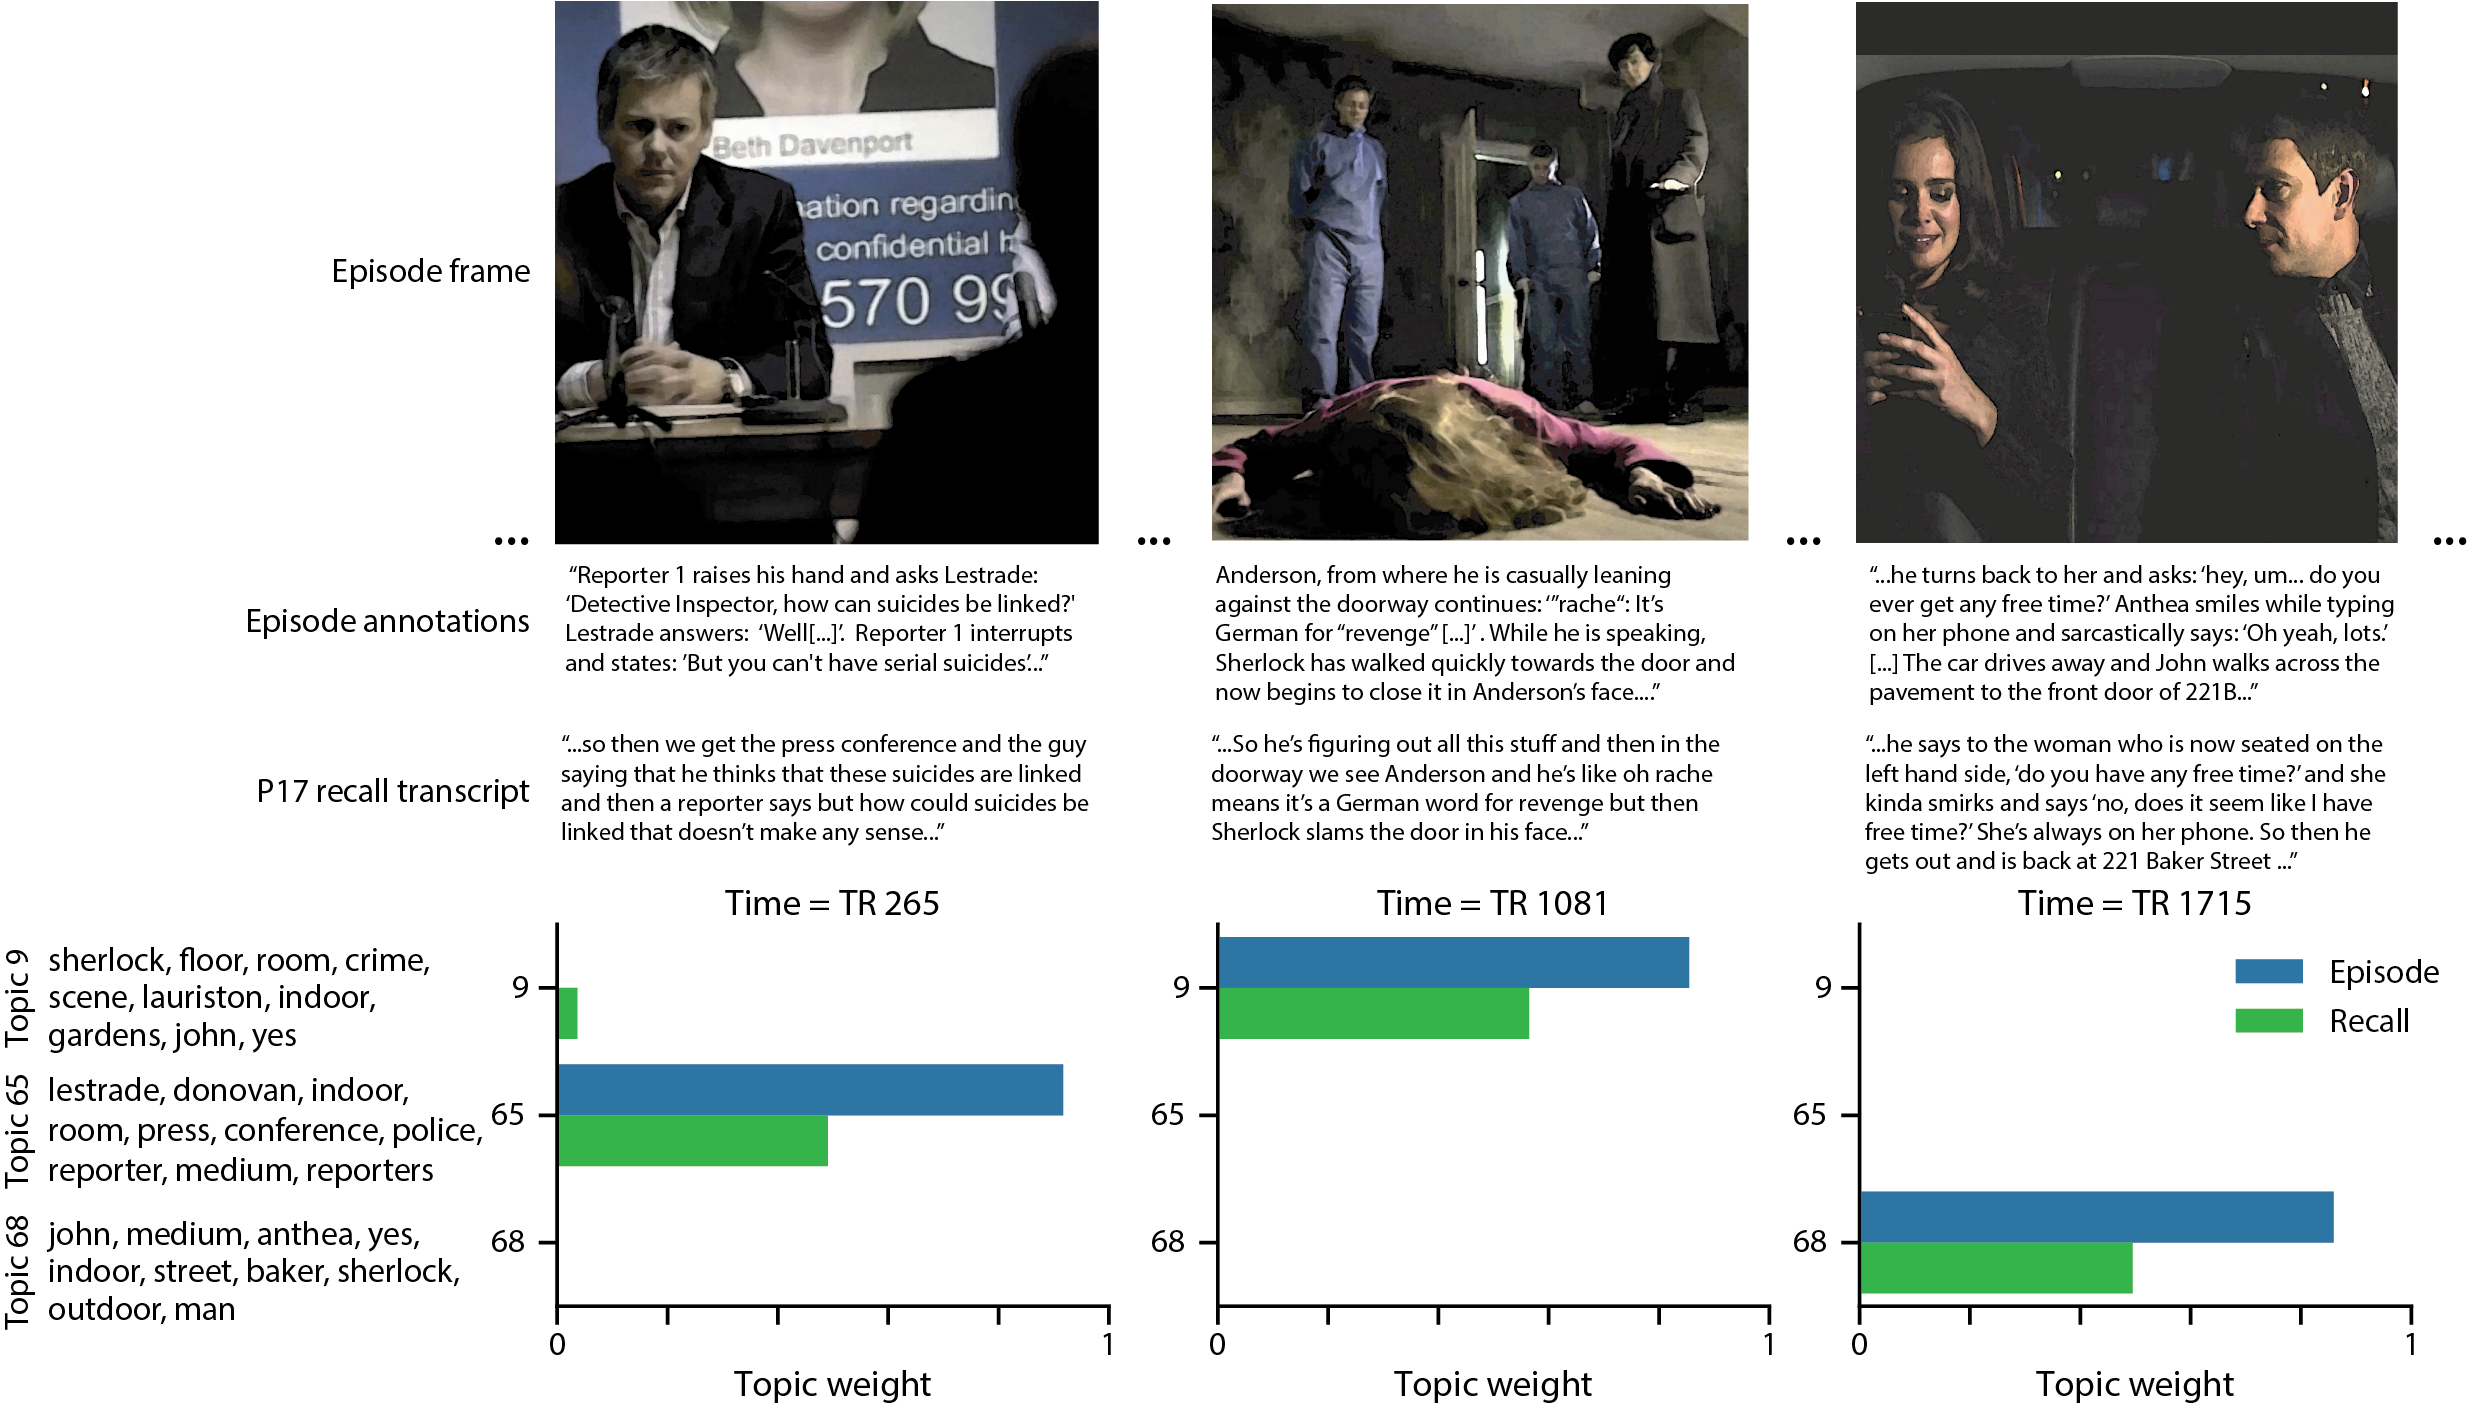
\includegraphics[width=1\textwidth]{figs/schematic}
\caption{\small \textbf{Topic weights in episode and recall content.} We used hand-annotated descriptions of each manually identified scene from the episode to fit a topic model.  Three example video frames (first row) and their associated descriptions (second row) are displayed.  The third row shows an example participant's later recalls of the same three scenes.  We used the topic model (fit to the episode annotations) to estimate topic vectors for each moment of the episode and each sentence of participants' recalls.  Example topic vectors are displayed in the bottom row (blue: episode annotations; green: example participant's recalls).  Three topic dimensions are shown (the highest-weighted topics for each of the three example scenes, respectively), along with the 10 highest-weighted words for each topic.  Figure~\topics~provides a full list of the top 10 words from each of the discovered topics.}
\label{fig:schematic}
\end{figure}
% add an x-label under the "

The 32 topics we found were heavily character-focused (i.e., the top-weighted word in each topic was nearly always a character) and could be roughly divided into themes centered around Sherlock Holmes (the titular character), John Watson (Sherlock's close confidant and assistant), supporting characters (e.g., Inspector Lestrade, Sergeant Donovan, or Sherlock's brother Mycroft), or the interactions between various groupings of these characters (see Fig.~\topics).  Several of the identified topics were highly similar, which we hypothesized might allow us to distinguish between subtle narrative differences if the distinctions between those overlapping topics were meaningful.  The topic vectors for each timepoint were also \textit{sparse}, in that only a small number (typically one or two) of topics tended to be ``active" in any given timepoint (see Fig.~\ref{fig:model}A).  Further, the dynamics of the topic activations appeared to exhibit \textit{persistence} (i.e., given that a topic was active in one timepoint, it was likely to be active in the following timepoint) along with \textit{occasional rapid changes} (i.e., occasionally topics would appear to spring into or out of existence).  These two properties of the topic dynamics may be seen in the block diagonal structure of the timepoint-by-timepoint correlation matrix (Fig.~\ref{fig:model}B) and reflect the gradual drift and sudden shifts fundamental to the temporal dynamics of real-world experiences.  Given this observation, we adapted an approach devised by \cite{BaldEtal17}, and used a hidden Markov model (HMM) to identify the \textit{event boundaries} where the topic activations changed rapidly (i.e., the boundaries of the blocks in the temporal correlation matrix; event boundaries identified by the HMM are outlined in yellow in Fig.~\ref{fig:model}B).  Part of our model fitting procedure required selecting an appropriate number of ``events" into which the topic trajectory should be segmented.  To accomplish this, we used an optimization procedure that maximized the difference between the topic weights for timepoints within an event versus timepoints across multiple events (see \textit{Methods} for additional details).  We then created a stable ``summary'' of the content within each episode event by averaging the topic vectors across the timepoints spanned by each event (Fig.~\ref{fig:model}C).

\begin{figure}[tp]
\centering
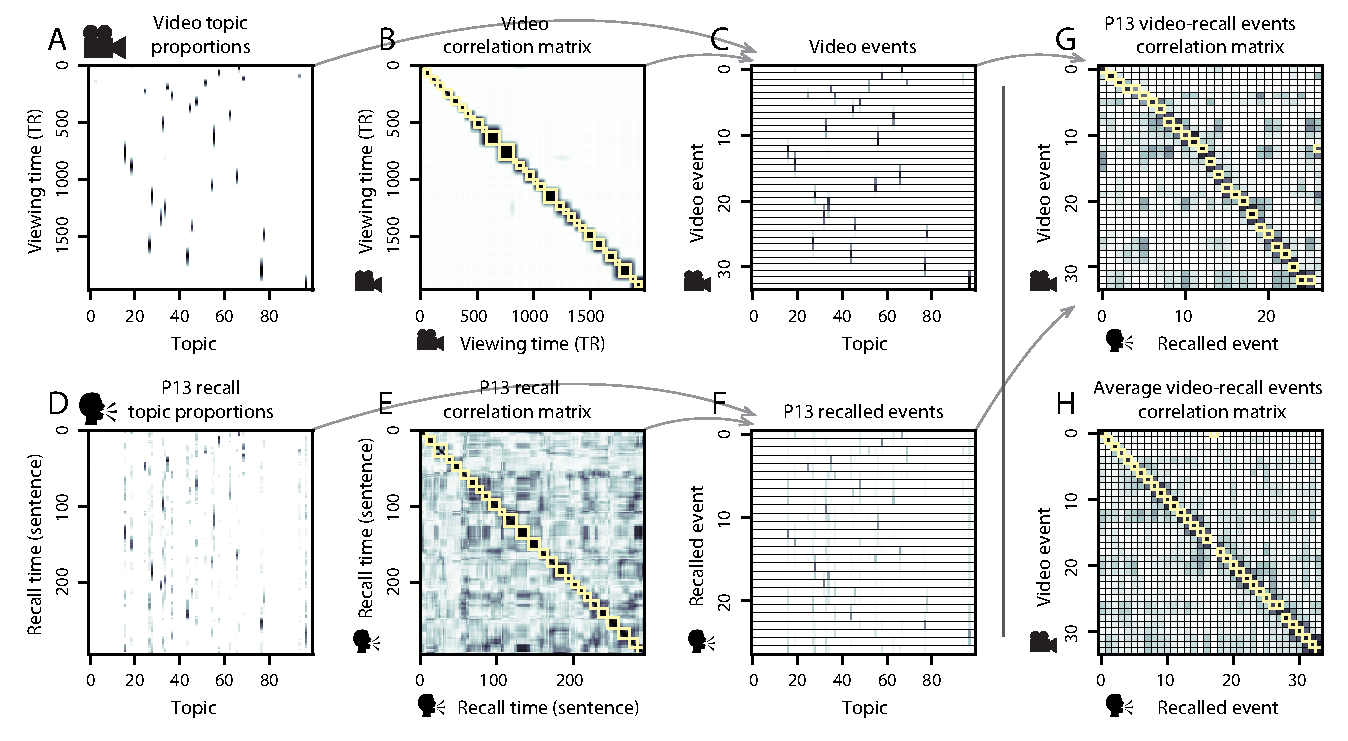
\includegraphics[width=\textwidth]{figs/eventseg}
\caption{\small \textbf{Modeling naturalistic stimuli and recalls.} All panels: darker colors indicate greater values; range: [0, 1].  \textbf{A.} Topic vectors ($K = 100$) for each of the 1976 episode timepoints.  \textbf{B.} Timepoint-by-timepoint correlation matrix of the topic vectors displayed in Panel A.  Event boundaries discovered by the HMM are denoted in yellow (30 events detected).  \textbf{C.} Average topic vectors for each of the 30 episode events. \textbf{D.} Topic vectors for each of 265 sliding windows of sentences spoken by an example participant while recalling the episode.  \textbf{E.} Timepoint-by-timepoint correlation matrix of the topic vectors displayed in Panel D. Event boundaries detected by the HMM are denoted in yellow (22 events detected).  For similar plots for all participants, see Figure~\corrmats.  \textbf{F.} Average topic vectors for each of the 22 recall events from the example participant.  \textbf{G.} Correlations between the topic vectors for every pair of episode events (Panel C) and recall events (from the example participant; Panel F).  For similar plots for all participants, see Figure~\matchmats.  \textbf{H.} Average correlations between each pair of episode events and recall events (across all 17 participants).  To create the figure, each recalled event was assigned to the episode event with the most correlated topic vector (yellow boxes in panels G and H).}
\label{fig:model}
\end{figure}
% I'm all for citing software packages, but where what's the distinction between packages we do cite (seaborn, brainiak, sklearn, hypertools, quail, umap, etc.) and don't cite (wordcloud, nilearn, fastdtw, etc.)?
% - Paxton
% I also flagged the seaborn reference for removal here. Def not critical to understanding the figure - Andy

Given that the time-varying content of the episode could be segmented cleanly into discrete events, we wondered whether participants' recalls of the episode also displayed a similar structure.  We applied the same topic model (already trained on the episode annotations) to each participant's recalls.  Analogously to how we parsed the time-varying content of the episode, to obtain similar estimates for each participant's recall, we treated each overlapping  window of (up to 10) sentences from their transcript as a ``document," and computed the most probable mix of topics reflected in each timepoint's sentences.  This yielded, for each participant, a number-of-windows by number-of-topics topic proportions matrix that characterized how the topics identified in the original episode were reflected in the participant's recalls.  Note that an important feature of our approach is that it allows us to compare participants' recalls to events from the original episode, despite different participants using widely varying language to describe the events, and that those descriptions often diverged in content and quality from the episode annotations.  This is a substantial benefit of projecting the episode and recalls into a shared ``topic'' space.  An example topic proportions matrix from one participant's recalls is shown in Figure~\ref{fig:model}D.

Although the example participant's recall topic proportions matrix has some visual similarity to the episode topic proportions matrix, the time-varying topic proportions for the example participant's recalls are not as sparse as those for the episode (compare Figs.~\ref{fig:model}A and D).  Similarly, although there do appear to be periods of stability in the recall topic dynamics (i.e., most topics are active or inactive over contiguous blocks of time), the changes in topic activations that define event boundaries appear less clearly delineated in participants' recalls than in the episode's annotations.  To examine these patterns in detail, we computed the timepoint-by-timepoint correlation matrix for the example participant's recall trajectory (Fig.~\ref{fig:model}E).  As in the episode correlation matrix (Fig.~\ref{fig:model}B), the example participant's recall correlation matrix has a strong block diagonal structure, indicating that their recalls are discretized into separated events.  As for the episode correlation matrix, we leveraged an HMM-based optimization procedure (see \textit{Methods}) to determine how many events are reflected in the participant's recalls and where specifically the event boundaries fall (outlined in yellow).  We carried out a similar analysis on all 17 participants' recall topic proportions matrices (Fig.~\corrmats).

Two clear patterns emerged from this set of analyses.  First, although every individual participant's recalls could be segmented into discrete events (i.e., every individual participant's recall correlation matrix exhibited clear block diagonal structure; Fig.~\corrmats), each participant appeared to have a unique \textit{recall resolution}, reflected in the sizes of those blocks.  While some participants' recall topic proportions segmented into just a few events (e.g., Participants P4, P5, and P7), others' segmented into many shorter duration events (e.g., Participants P12, P13, and P17).  This suggests that different participants may be recalling the episode with different levels of detail---i.e., some might touch on just the major plot points, whereas others might attempt to recall every minor scene or action.  The second clear pattern present in every individual participant's recall correlation matrix was that, unlike in the episode correlation matrix, there were substantial off-diagonal correlations.  Whereas each event in the original episode was (largely) separable from the others (Fig.~\ref{fig:model}B), in transforming those separable events into memory, participants appeared to be integrating across multiple events, blending elements of previously recalled and not-yet-recalled content into each newly recalled event~\citep[Figs.~\ref{fig:model}E, \corrmats; also see][]{MannEtal11, HowaEtal12, Mann19}.

The above results indicate that both the structure of the original episode and participants' recalls of the episode exhibit event boundaries that can be identified automatically by characterizing the dynamic content using a shared topic model and segmenting the content into events via HMMs.  Next, we asked whether some correspondence might be made between the specific content of the events the participants experienced in the episode, and the events they later recalled.  One approach to linking the experienced (episode) and recalled events is to label each recalled event as matching the episode event with the most similar (i.e., most highly correlated) topic vector (Figs.~\ref{fig:model}G, \matchmats).  This yields a sequence of ``presented" events from the original episode, and a (potentially differently ordered) sequence of ``recalled" events for each participant.  Analogous to classic list-learning studies, we can then examine participants' recall sequences by asking which events they tended to recall first~\citep[probability of first recall; Fig.~\ref{fig:list-learning}A;][]{AtkiShif68, PostPhil65, WelcBurn24}; how participants most often transition between recalls of the events as a function of the temporal distance between them~\citep[lag-conditional response probability; Fig.~\ref{fig:list-learning}B;][]{Kaha96}; and which events they were likely to remember overall~\citep[serial position recall analyses; Fig.~\ref{fig:list-learning}C;][]{Murd62a}. Interestingly, for two of these analyses (probability of first recall and lag-conditional response probability curves) we observed patterns comparable to classic effects from list-learning literature: namely, a higher probability of initiating recall with the first event in the sequence (Fig.~\ref{fig:list-learning}A) and a higher probability of transitioning to neighboring events with an asymmetric forward bias (Fig.~\ref{fig:list-learning}B). In contrast, we did not observe a pattern comparable to the serial position effect (Fig.~\ref{fig:list-learning}C), but rather greater memory for specific events distributed approximately evenly throughout the episode.

We can also apply two list-learning-native analyses that describe how participants group items in their recall sequences: temporal clustering and semantic clustering \citep[][see \textit{Methods} for details]{PolyEtal09}.~Temporal clustering refers to the extent to which participants group their recall responses according to encoding position.  Overall, we found that sequentially viewed episode events were clustered heavily in participants' recall event sequences (mean clustering score: 0.767, SEM: 0.029), and that participants with higher temporal clustering scores tended to perform better according to both \cite{ChenEtal17}'s hand-annotated memory scores (Pearson's $r(15) = 0.62,~p = 0.008$) and our model's estimate (Pearson's $r(15) = 0.54,~p = 0.024$).  Semantic clustering measures the extent to which participants cluster their recall responses according to semantic similarity.  We found that participants tended to recall semantically similar episode events together (mean clustering score: 0.787, SEM: 0.018), and that semantic clustering score was also related to both hand-annotated  (Pearson's $r(15) = 0.65,~p = 0.004$) and model-derived (Pearson's $r(15) = 0.63,~p = 0.007$) memory performance.
% NOTE:
% Semantic and temporal clustering are both positively correlated with n_events -- r=0.49; p=0.046 and r=0.61; p=0.009, respectively.
% - Paxton

\begin{figure}[t]
  \centering
  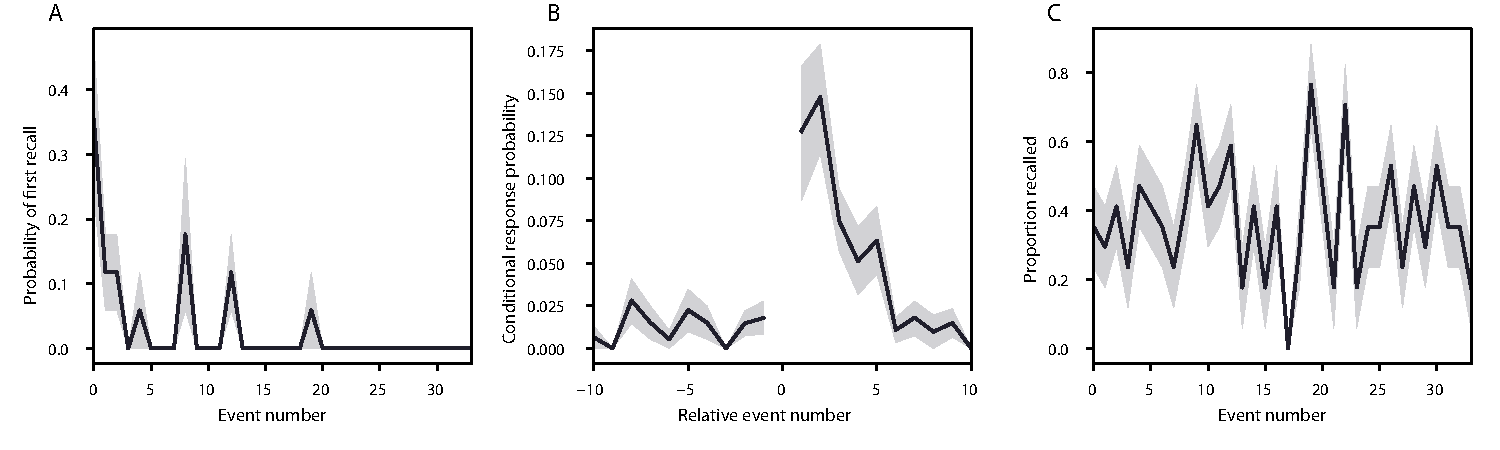
\includegraphics[width=1\textwidth]{figs/list_learning}
  \caption{\small \textbf{Naturalistic extensions of classic list-learning memory analyses.} \textbf{A.} The probability of first recall as a function of the serial position of the event in the episode. \textbf{B}.  The probability of recalling each event, conditioned on having most recently recalled the event \textit{lag} events away in the episode.  \textbf{C.} The proportion of participants who recalled each event, as a function of the serial position of the events in the episode.  All panels: error ribbons denote bootstrap-estimated standard error of the mean.}
  \label{fig:list-learning}
\end{figure}

\begin{figure}[t]
  \centering
  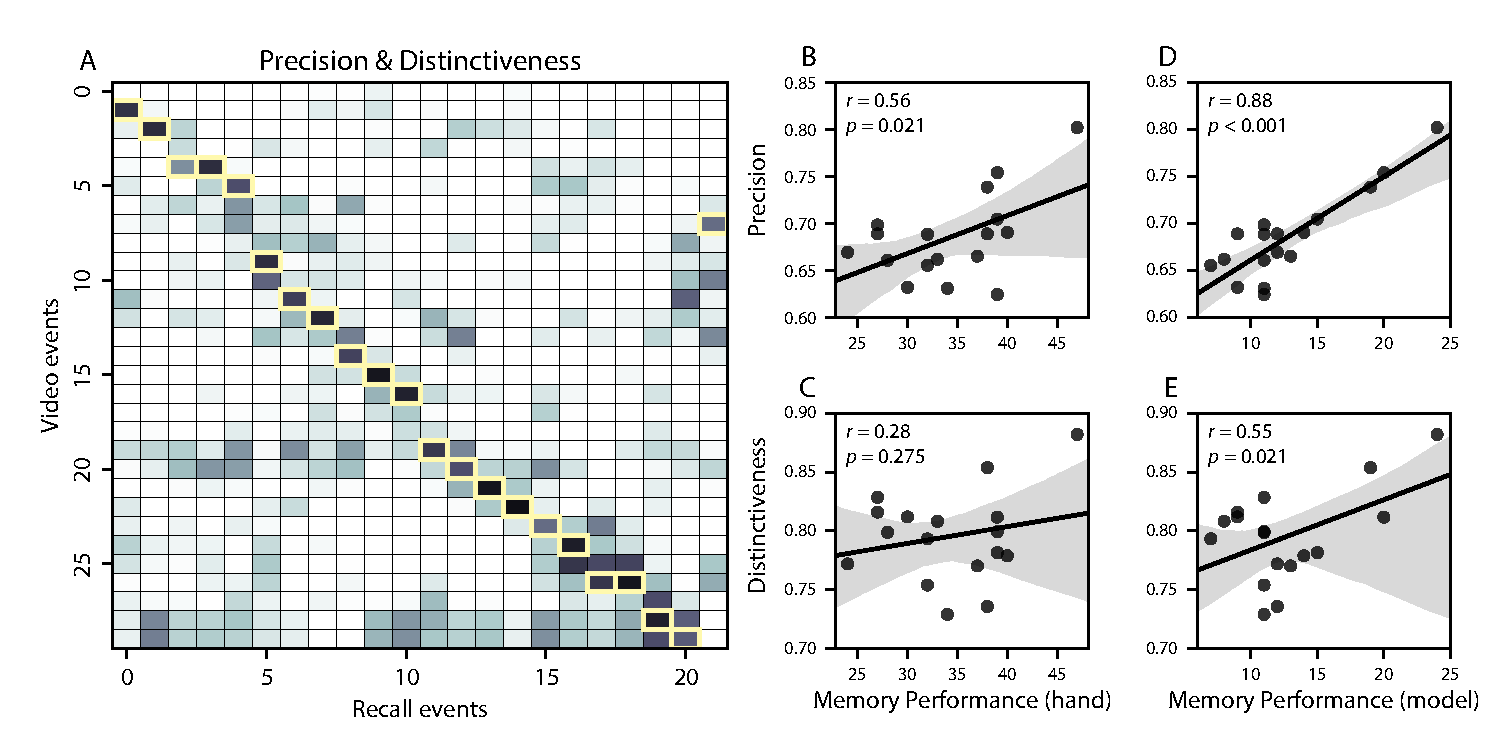
\includegraphics[width=1\textwidth]{figs/precision_distinctiveness}
  \caption{\small \textbf{Novel content-based metrics of naturalistic memory: precision and distinctiveness.} \textbf{A.} The episode-recall correlation matrix for a representative participant (17).  The yellow boxes highlight the maximum correlation in each column.  The example participant's overall precision score was computed as the average across correlation values in the yellow boxes.  Their distinctiveness score was computed as the average (over recall events) of 1 minus the average correlation between each recall event and all other recall events that do not display a box in the same row.  \textbf{B.} The (Pearson's) correlation between precision and hand-annotated memory performance. \textbf{C.} The correlation between distinctiveness and hand-annotated memory performance. \textbf{D.} The correlation between precision and the number of episode events successfully recalled, as determined by our model. \textbf{E.} The correlation between distinctiveness and the number of episode events successfully recalled, as determined by our model.}
  \label{fig:precision-distinctiveness}
\end{figure}
% Need to reconcile the description of distinctiveness with how we computed it... - Andy

Statistical models of memory studies often treat recall success as binary (in other words, an item either was or was not recalled), or occasionally categorical \citep[e.g., to distinguish familiarity from recollection;][]{YoneEtal02}.  Such approaches are tenable in classical list-learning or recognition memory paradigms, as the presented stimuli tend to be very simple (e.g., a sequence of individual words or items).  However, memory for naturalistic experiences is much more nuanced.  For example, certain aspects of an experience might be correctly remembered at varying levels of detail, or distorted, or forgotten entirely.  Further, each remembering is itself a richly structured phenomenon.  Our framework produces a content-based model of individual episode and recall events by projecting the dynamic content of the episode and participants' recalls into a shared topic space.  This allows for direct, quantitative comparisons between all stimulus and recall events, as well as between the recall events themselves.  Leveraging these content-based models of the stimulus/recall events, we developed two novel, \textit{continuous} metrics for analyzing naturalistic memory:~\textit{precision} and \textit{distinctiveness}.  Precision is intended to capture the ``completeness'' of recall, or how fully the presented content was recapitulated in memory.  We define a recall event's precision as the maximum correlation between the topic proportions of that recall event and any episode event (Fig.~\ref{fig:precision-distinctiveness}).  A second novel metric we introduce here is \textit{distinctiveness}, which is intended to capture the ``specificity'' of recall.  In other words, distinctiveness quantifies the extent to which a given recalled event reflects the most similar presented event moreso than it does other presented events.  To compute a recall event's distinctiveness, we first identify the episode event to which its topic vector is most strongly correlated.  We then define distinctiveness as one minus the average correlation between the given recall event and all \textit{other} episode events.  In addition to individual events, one may also use these metrics to describe each participant's overall performance by averaging across a participant's event-wise precision or distinctiveness scores.  Participants whose recall events are more veridical descriptions of what happened in the episode event will presumably have higher precision scores. We find that, across participants, higher precision scores are positively correlated with both hand-annotated memory performance (as collected by Chen et al., 2017; Pearson's $r(15) = 0.60, p = 0.010$) and the number of episode events successfully remembered, as determined by our model (Pearson's $r(15) = 0.90, p < 0.001$).  We also hypothesized that participants who recounted events in a more distinctive way would display better overall memory.  We find that participants' distinctiveness scores were positively
correlated with our model's estimated number of recall events (Pearson's $r(15) = 0.55, p = 0.021$).  However, we found no evidence that distinctiveness scores were correlated with hand-annotated memory performance (Pearson's $r(15) = 0.28, p = 0.275$).  We elaborate on this potential discrepency in the \textit{Discussion} section.

\begin{figure}[t]
  \centering
  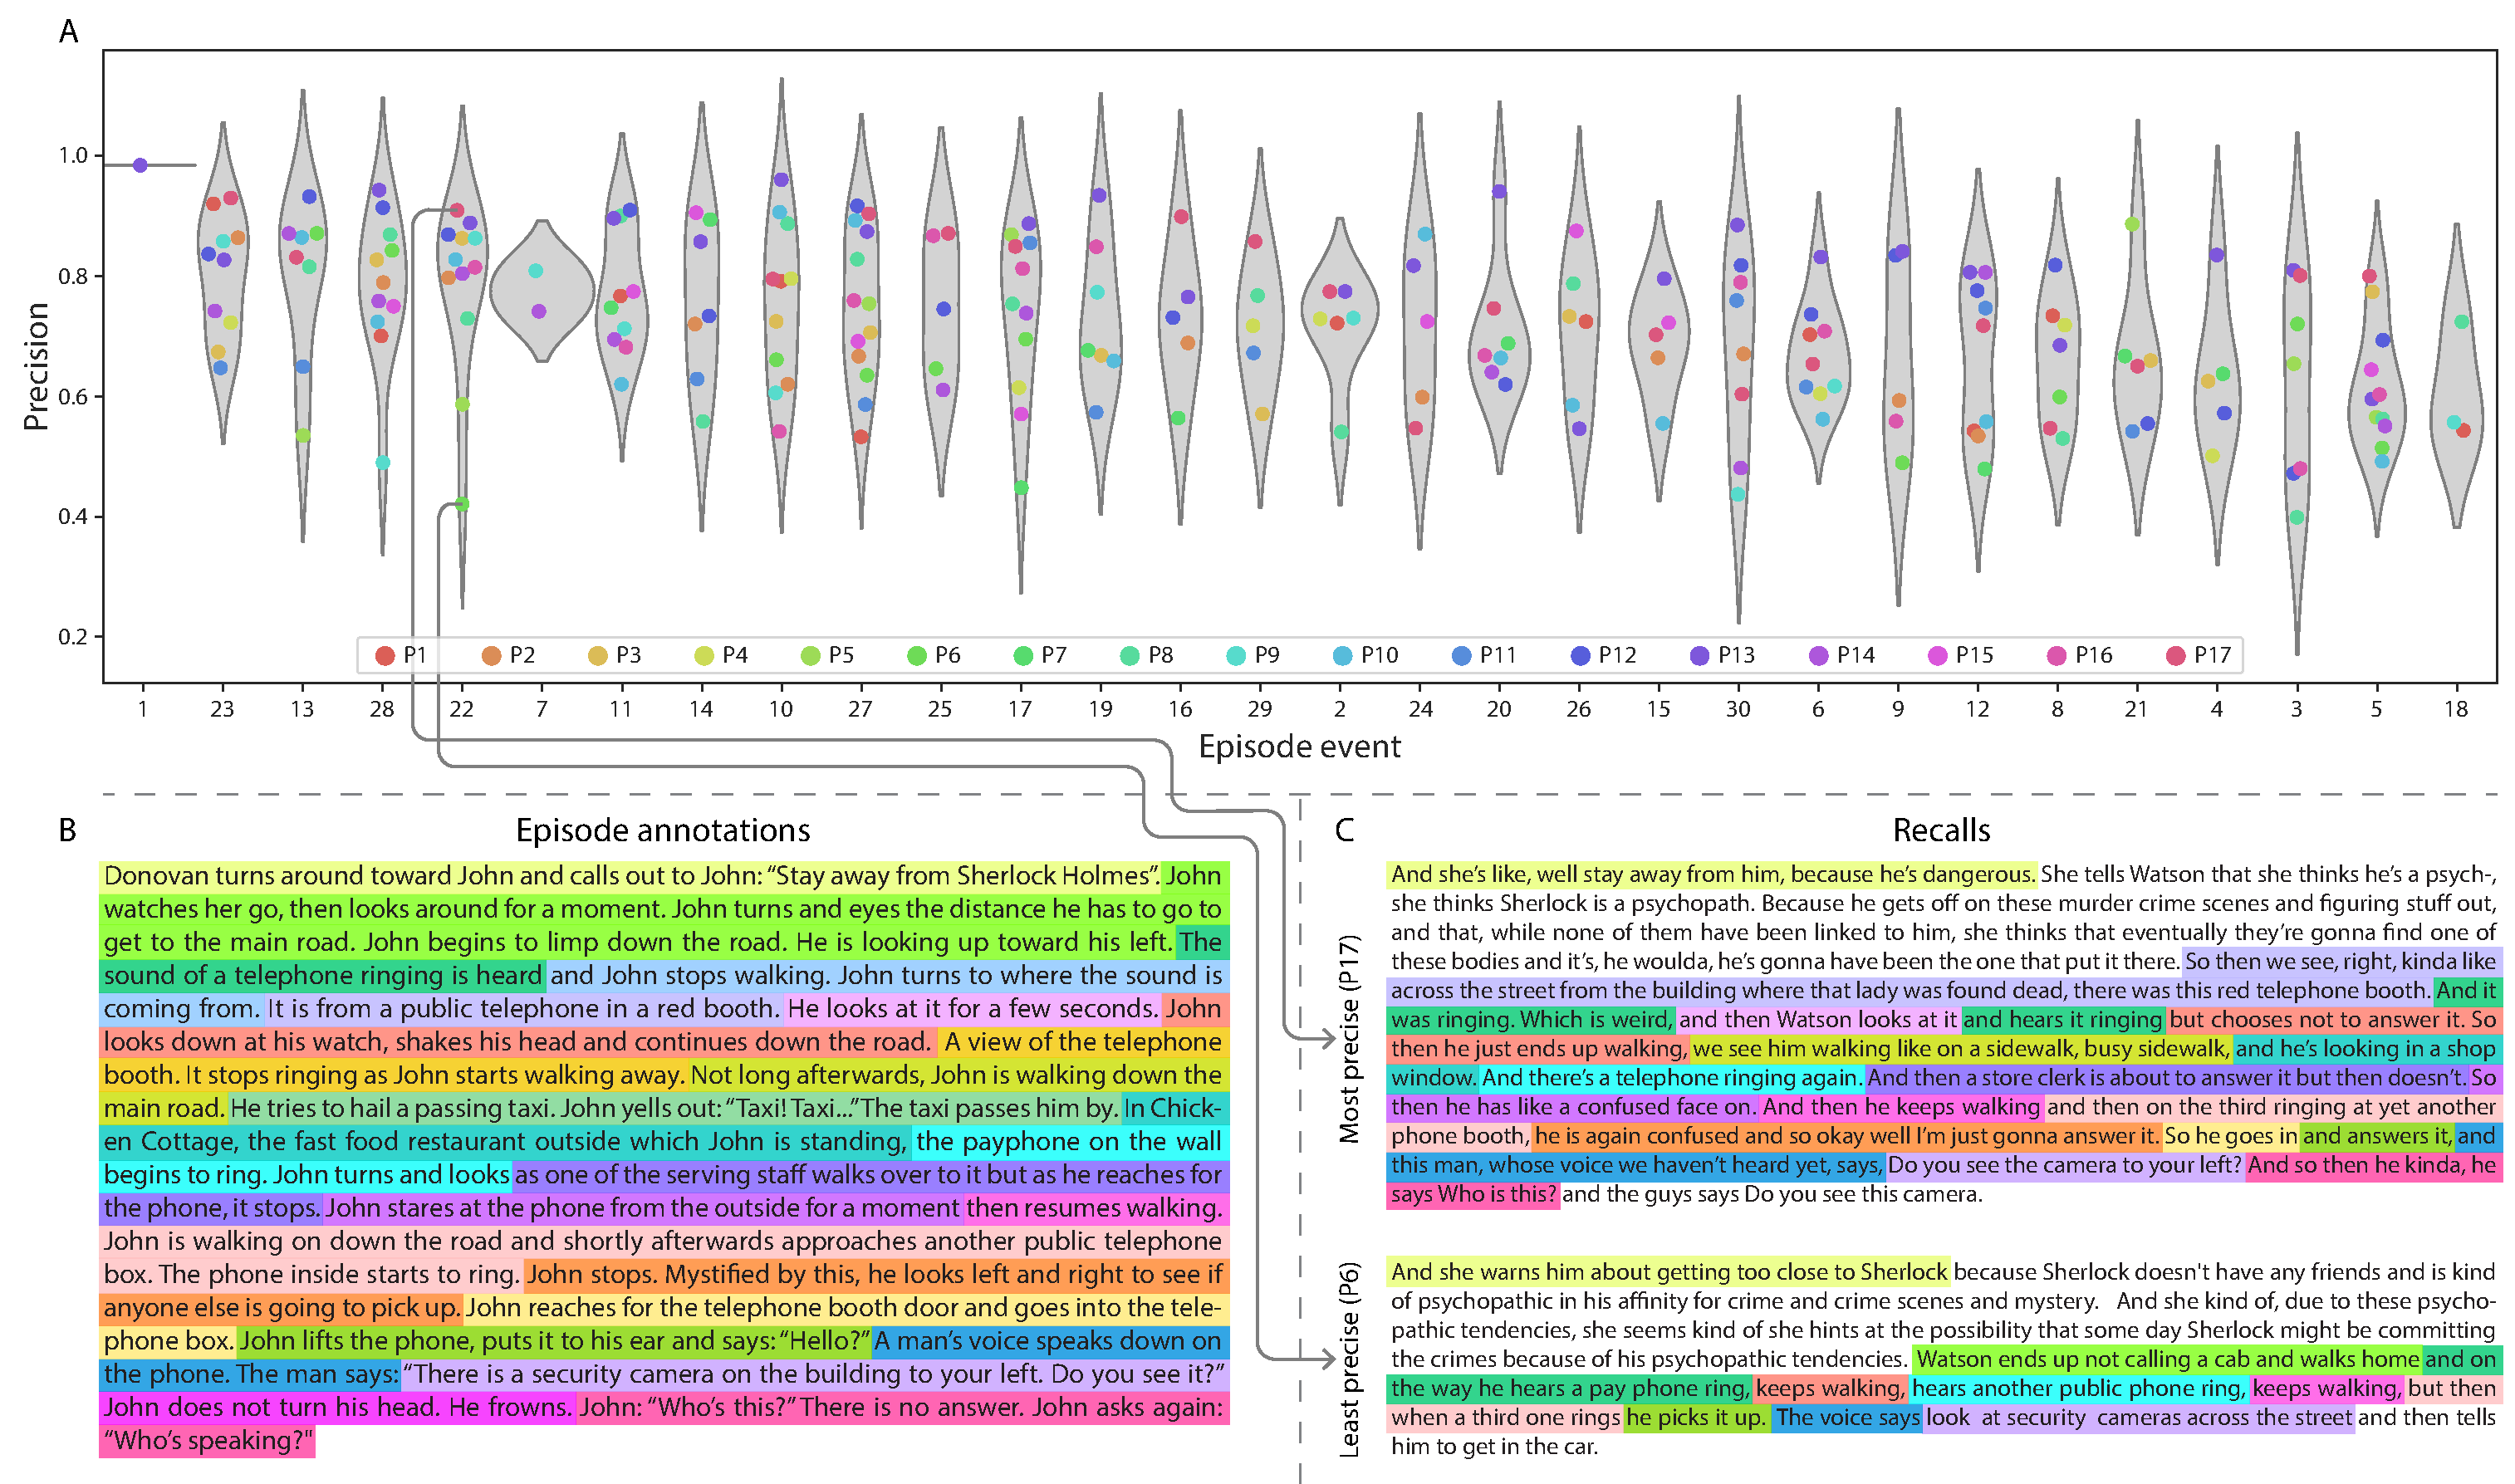
\includegraphics[width=1\textwidth]{figs/precision_detail}
  \caption{\small \textbf{Precision metric reflects completeness of recall.} \textbf{A.} Recall precision by episode event.  Grey violin plots display kernel density estimates for the distribution of recall precision scores for a single episode event.  Colored dots within each violin plot represent individual participants' recall precision for the given event.  episode events are ordered along the $x$-axis by the average precision with which they were remembered.  \textbf{B.} The set of ``Narrative Details" episode annotations (generated by \citealp{ChenEtal17}) for scenes comprising an example episode event (22) identified by the HMM.  Each action or feature is highlighted in a different color.  \textbf{C.} A subset of the sentences comprising the most precise (P17) and least precise (P6) participants' recalls of episode event 22.  Descriptions of specific actions or features reflecting those highlighted in panel B are highlighted in the corresponding color.}
  \label{fig:precision-detail}
\end{figure}

\begin{figure}[t]
  \centering
  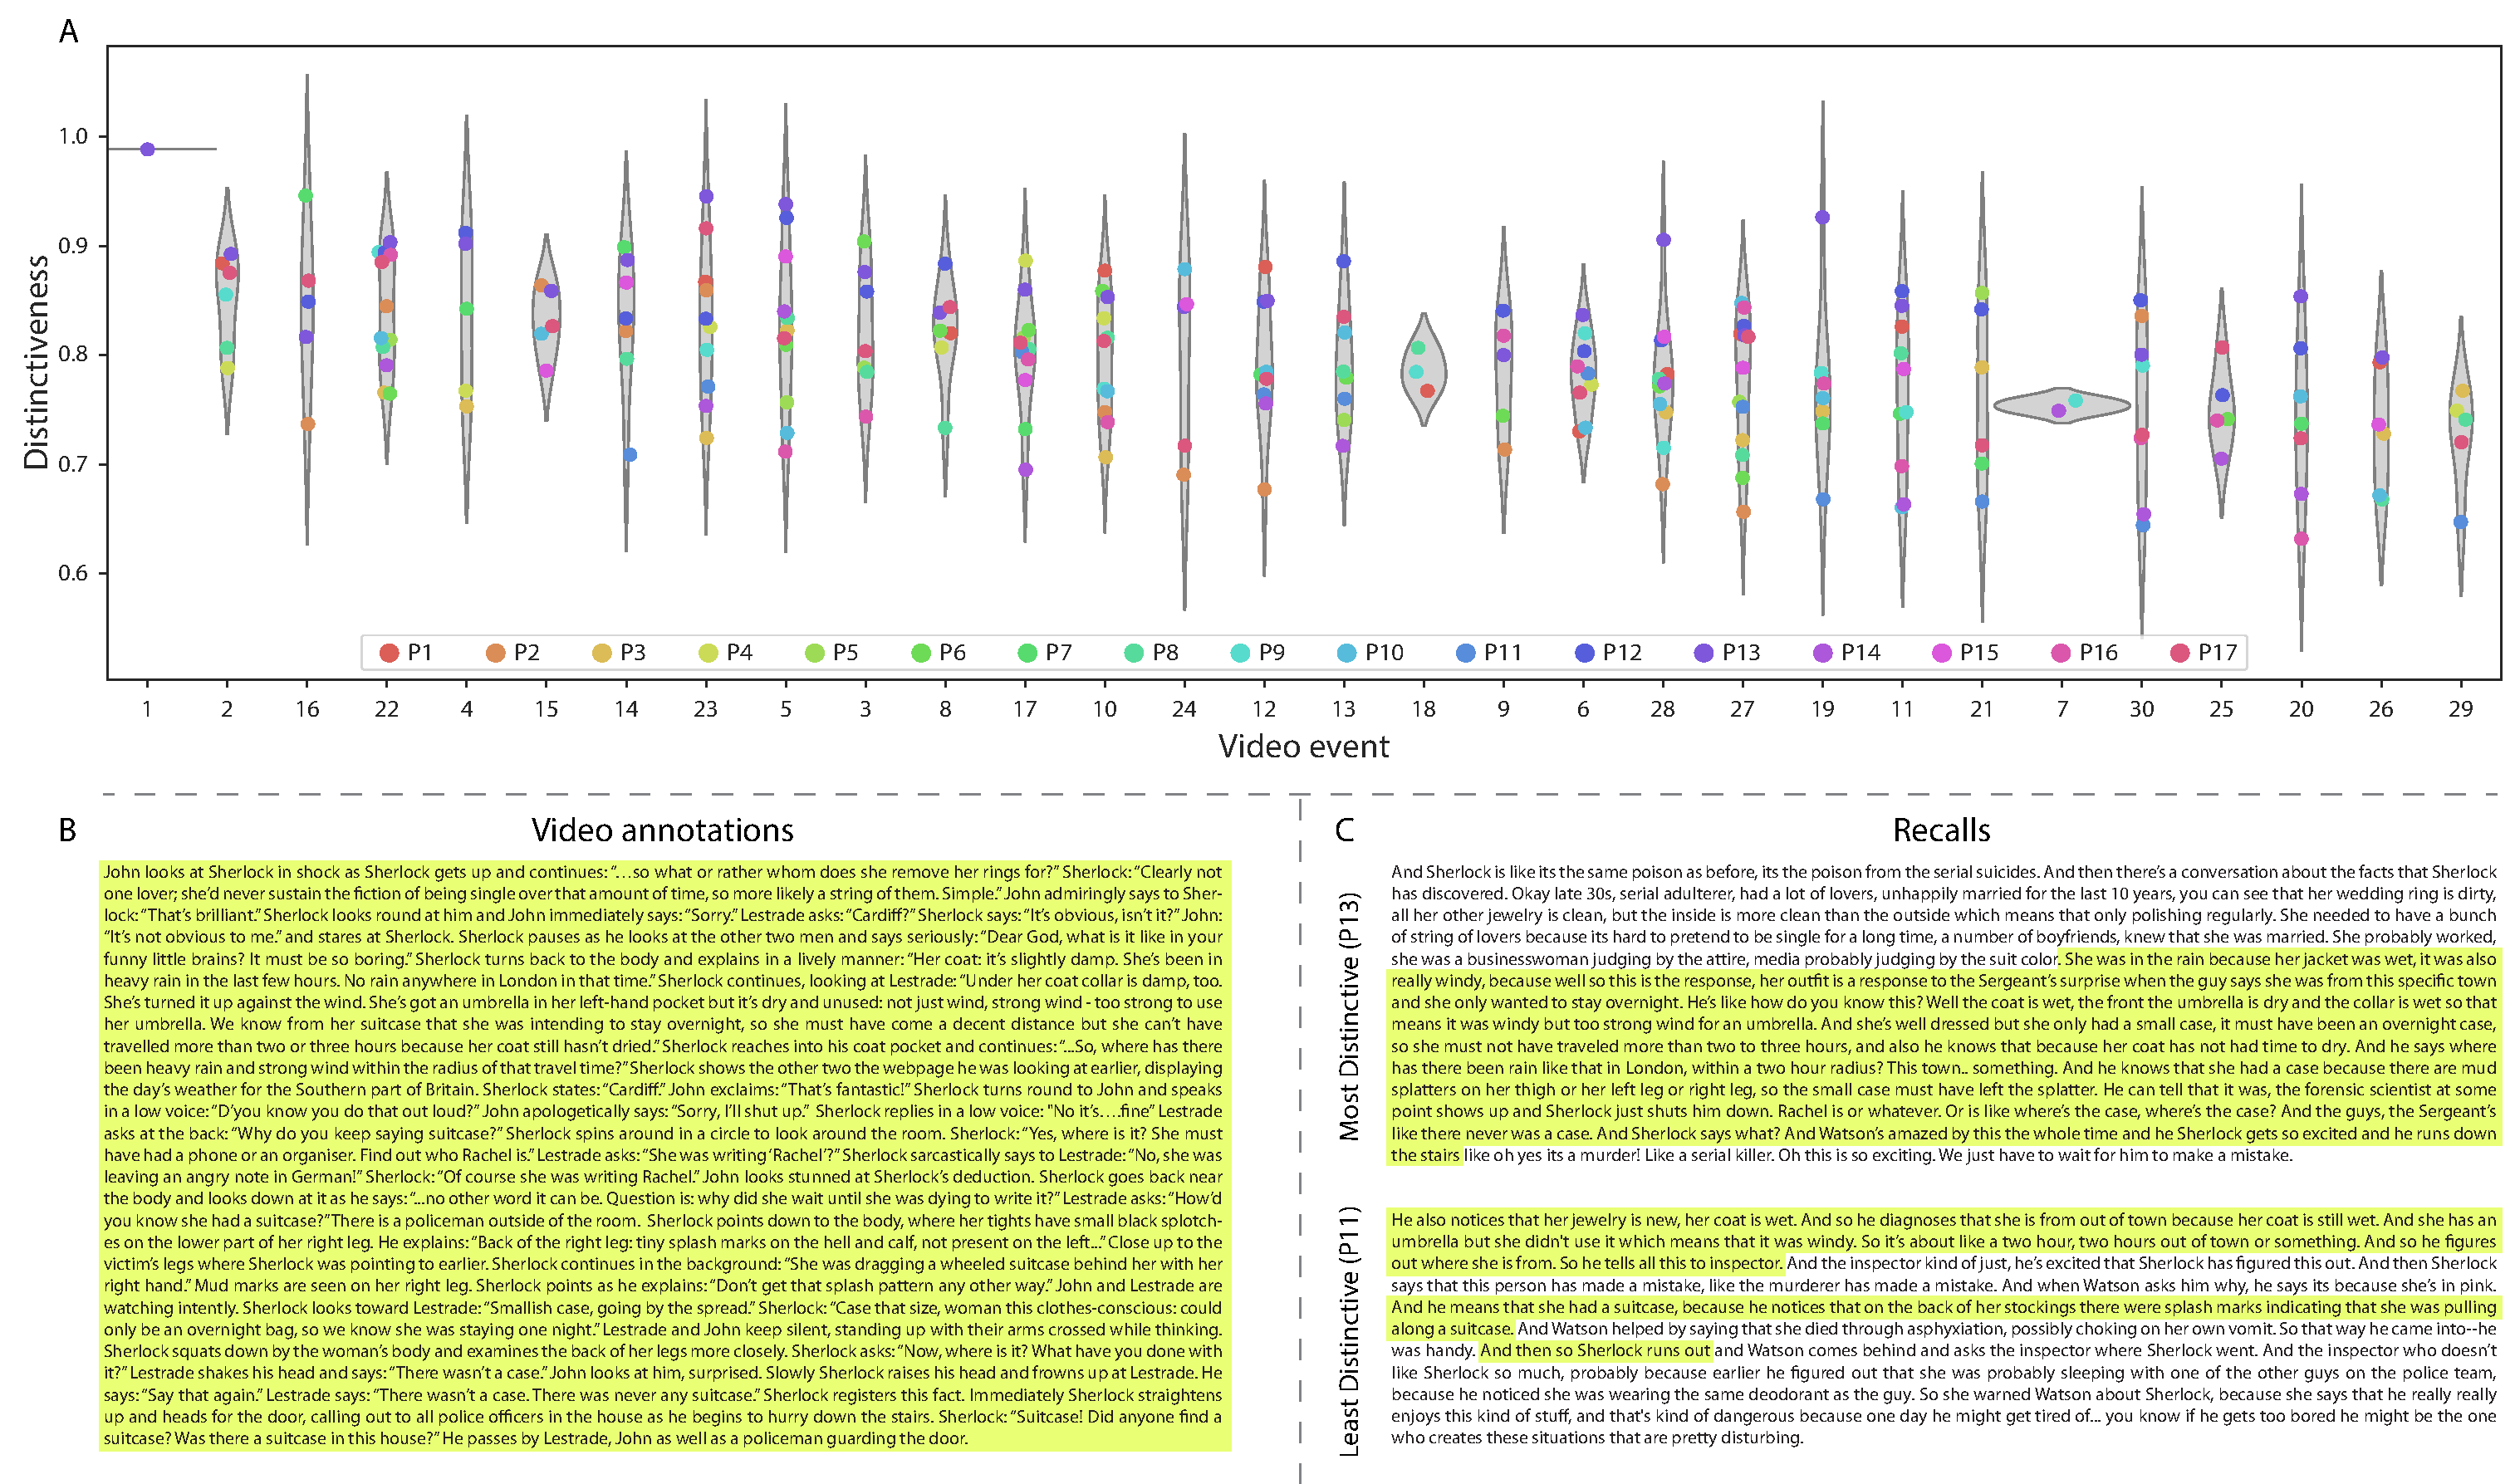
\includegraphics[width=1\textwidth]{figs/distinctiveness_detail}
  \caption{\small \textbf{Distinctiveness metric reflects specificity of recall.} \textbf{A.} Recall distinctiveness by episode event.  Kernel density estimates for each episode event's distribution of recall distinctiveness scores, analogous to Fig.~\ref{fig:precision-detail}A.  \textbf{B.} The sets of ``Narrative Details" episode annotations (generated by \citealp{ChenEtal17}) for scenes comprising episode events described by the example participants in panel C.  Each event's text is highlighted in a different color.  \textbf{C.} The sentences comprising the most distinctive (P13) and least distinctive (P11) participants' recalls of episode event 19.  Sections of recall describing each each episode event in panel B are highlighted with the corresponding color.}
  \label{fig:distinctiveness-detail}
\end{figure}

Further intuition for the behaviors captured by these two metrics may be gained by directly examining the content of the episode and recalls our framework models.  In Figure \ref{fig:precision-detail}, we contrast recalls for the same episode event (event 22) from two participants: one with a high precision score (P17), the other with a low precision score (P6).  From the HMM-identified event boundaries, we recovered the set of annotations describing the content of an example episode event (Fig.~\ref{fig:precision-detail}B), and divided them into different color-coded sections for each action or feature described.  We then similarly recovered the set of sentences comprising the corresponding recall event for each of the two example participants.  Because the recall sliding windows overlap heavily, and each recall event spans multiple recall timepoints (i.e., windows), we have stripped any sentences from the beginning and end that describe earlier or later episode events for the sake of readability.  In other words, Fig.~\ref{fig:precision-detail}C shows a subset of the full recall event text, comprising sentences between the first and last descriptions of content from the example episode event.  We then colored all words describing actions and features coded in panel B by their corresponding color.  Visual comparison of these example transcripts reveals that the more precise recall captures more of the episode event's content, and with more detail.

Figure \ref{fig:distinctiveness-detail} similarly contrasts two example participants' recalls for a common episode event (event 19) to illustrate the tangible differences between high and low distinctiveness scores.  Here, we have extracted the full set of sentences comprising the most distinctive recall event (P13) and least distinctive recall event (P11) matched to the example episode event (Fig.~\ref{fig:distinctiveness-detail}C).  We also extracted the annotations for the example episode event, as well as those from each other episode event whose content the example participants' single recall events described (Fig.~\ref{fig:distinctiveness-detail}B).  We then shaded the annotation text for each episode event with a different color, and shaded each word of the example participants' recall text by the color of the episode event it describes.  The majority of the most distinctive recall event text describes episode event 19's content, with the first five and last one sentence describing the episode events immediately preceding and succeeding the current one, respectively.  In contrast, the least distinctive recall of episode event 19 blends the content from five separate episode events, does not transition between them in order, and often combines descriptions of two episode events' content in the same sentence.

The prior analyses leverage the correspondence between the 100-dimensional topic proportion matrices for the episode and participants' recalls to characterize recall.  However, it is difficult to gain deep insights into the content of (or relationships between) experiences and memories solely by examining these topic proportions (e.g., Figs.~\ref{fig:model}A, D) or the corresponding correlation matrices (Figs.~\ref{fig:model}B, E, \corrmats).  And while we can directly examine the original text underlying these topic vectors (e.g., Figs.~\ref{fig:precision-detail},~\ref{fig:distinctiveness-detail}) to show how relationships between them reflect real-world behavior, this comparison becomes prohibitively cumbersome at larger timescales.  To visualize the time-varying high-dimensional content in a more intuitive way~\citep{HeusEtal18a}, we projected the topic proportions matrices onto a two-dimensional space using Uniform Manifold Approximation and Projection~\citep[UMAP; ][]{McInEtal18}.  In this lower-dimensional space, each point represents a single episode or recall event, and the distances between the points reflect the distances between the events' associated topic vectors (Fig.~\ref{fig:trajectory}). In other words, events that are nearer to each other in this space are more semantically similar, and those that are farther apart are less so.


\begin{figure}[tp]
\centering
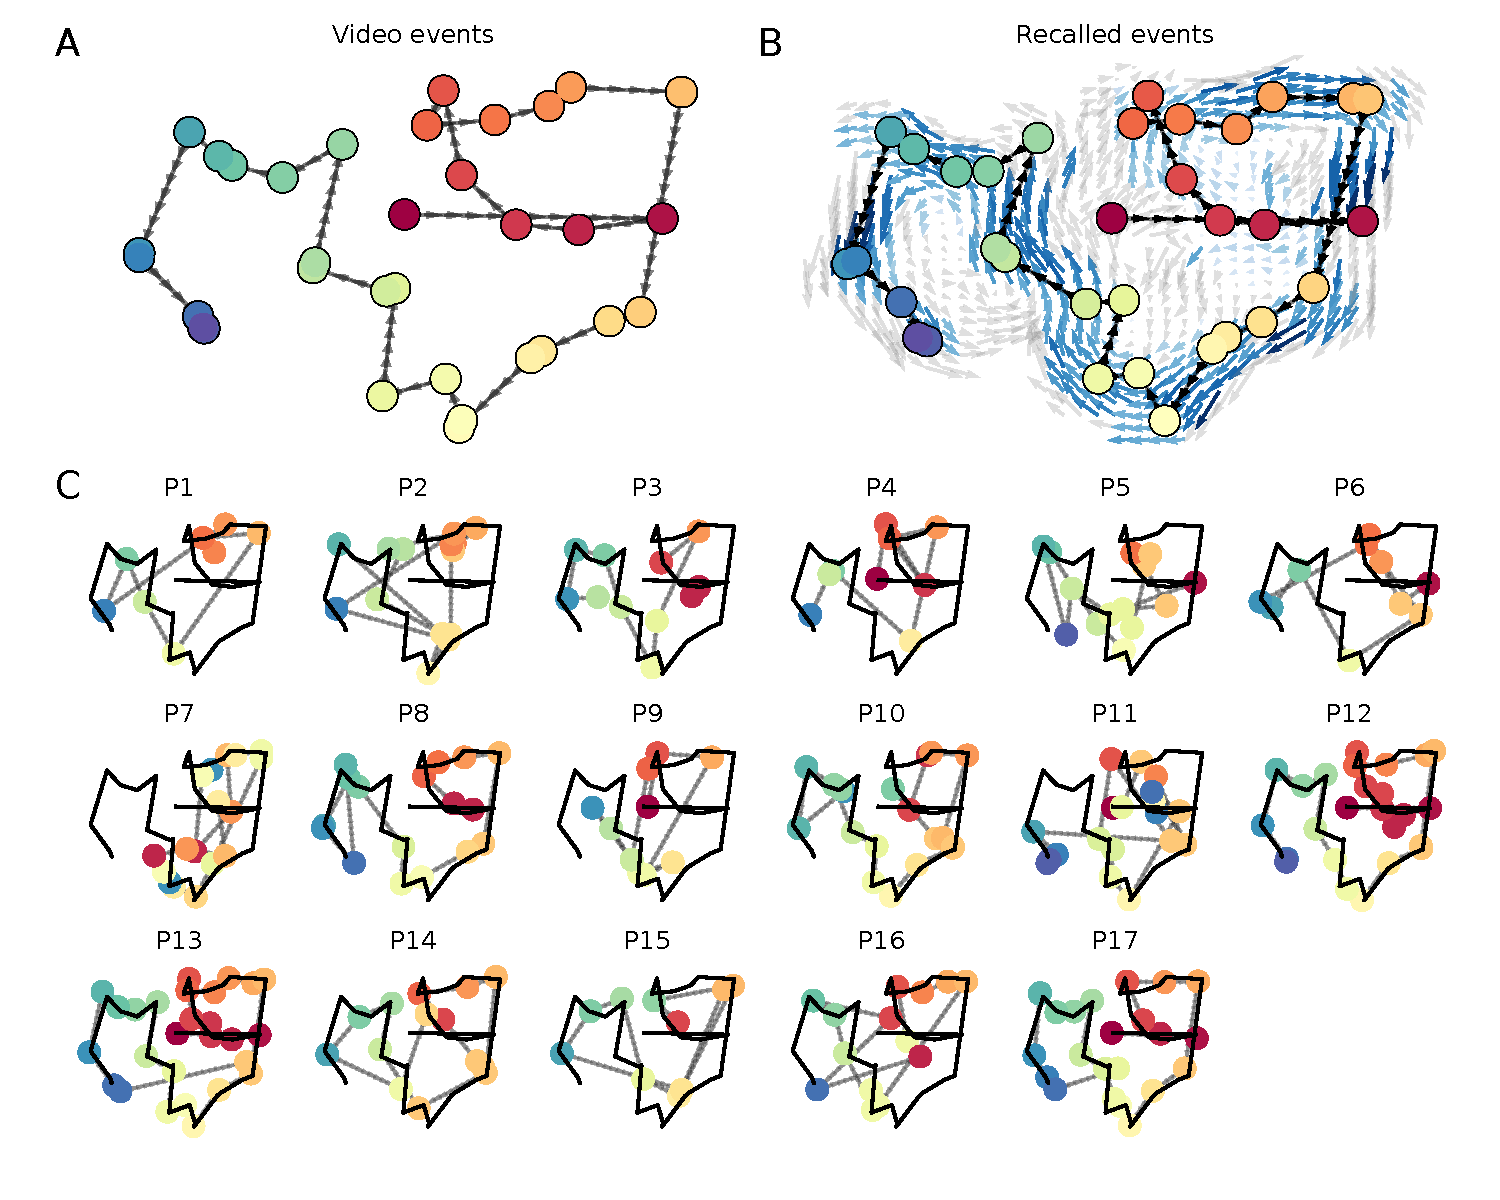
\includegraphics[width=1\textwidth]{figs/trajectory}
\caption{\small \textbf{Trajectories through topic space capture the dynamic content of the episode and recalls.}  All panels: the topic proportion matrices have been projected onto a shared two-dimensional space using UMAP.  \textbf{A.} The two-dimensional topic trajectory taken by the episode of \textit{Sherlock}.  Each dot indicates an event identified using the HMM (see \textit{Methods}); the dot colors denote the order of the events (early events are in red; later events are in blue), and the connecting lines indicate the transitions between successive events.  \textbf{B.} The average two-dimensional trajectory captured by participants' recall sequences, with the same format and coloring as the trajectory in Panel A.  To compute the event positions, we matched each recalled event with an event from the original episode (see \textit{Results}), and then we averaged the positions of all events with the same label.  The arrows reflect the average transition direction through topic space taken by any participants whose trajectories crossed that part of topic space; blue denotes reliable agreement across participants via a Rayleigh test ($p < 0.05$, corrected).  \textbf{C.} The recall topic trajectories (gray) taken by each individual participant (P1--P17).  The episode's trajectory is shown in black for reference.  Here, events (dots) are colored by their matched episode event (Panel A).}
\label{fig:trajectory}
\end{figure}


Visual inspection of the episode and recall topic trajectories reveals a striking pattern.  First, the topic trajectory of the episode (which reflects its dynamic content; Fig.~\ref{fig:trajectory}A) is captured nearly perfectly by the averaged topic trajectories of participants' recalls (Fig.~\ref{fig:trajectory}B).  To assess the consistency of these recall trajectories across participants, we asked: given that a participant's recall trajectory had entered a particular location in the reduced topic space, could the position of their \textit{next} recalled event be predicted reliably?  For each location in the the reduced topic space, we computed the set of line segments connecting successively recalled events (across all participants) that intersected that location (see \textit{Methods} for additional details).  We then computed (for each location) the distribution of angles formed by the lines defined by those line segments and a fixed reference line (the $x$-axis).  Rayleigh tests revealed the set of locations in topic space at which these across-participant distributions exhibited reliable peaks (blue arrows in Fig.~\ref{fig:trajectory}B reflect significant peaks at $p < 0.05$, corrected).  We observed that the locations traversed by nearly the entire episode trajectory exhibited such peaks.  In other words, participants exhibited similar trajectories that also matched the trajectory of the original episode (Fig.~\ref{fig:trajectory}C).  This is especially notable when considering the fact that the number of events participants recalled (dots in Fig.~\ref{fig:trajectory}C) varied considerably across people, and that every participant used different words to describe what they had remembered happening in the episode.  Differences in the numbers of remembered events appear in participants' trajectories as differences in the sampling resolution along the trajectory.  We note that this framework also provides a means of disentangling classic ``proportion recalled'' measures (i.e., the proportion of episode events described in participants' recalls) from participants' abilities to recapitulate the overall unfolding of the original episode's content (i.e., the similarity between the shapes of the original episode trajectory and that defined by each participant's recounting of the episode).
% ------ NOTE: ------
% not sure it's accurate to use "topic space" in paragraph above.  These analyses were all conducted in the 2D manifold space
% - Paxton
% I added "reduced" before the first reference and second reference to topic space to make it clear the analyses were performed on the 2D space. - Andy

In addition to the more ``holistic'' measure of memory described in the previous section, our framework also affords the ability to drill down to individual words and quantify how each word relates to the  memorability of each event. The results displayed in Figures \ref{fig:list-learning}C and \ref{fig:precision-detail}A suggest that certain events were remembered better than others.  Given this, we next asked asked whether the events were generally remembered well or poorly tended to reflect particular content.  Because our analysis framework projects the dynamic episode content and participants' recalls into a shared space, and because the dimensions of that space represent topics (which are, in turn, sets of weights over known words in the vocabulary), we are able to recover the weighted combination of words that make up any point (i.e., topic vector) in this space.  We first computed the average precision with which participants recalled each of the 30 episode events (Fig.~\ref{fig:topics}A; note that this result is analogous to a serial position curve created from our continuous recall quality metric).  We then computed a weighted average of the topic vectors for each episode event, where the weights reflected how reliably each event was recalled.  To visualize the result, we created a ``wordle'' image~\citep{MuelEtal18} where words weighted more heavily by better-remembered topics appear in a larger font (Fig.~\ref{fig:topics}B, green box).  Across the full episode, content that reflected topics necessary to convey the central focus of the episode (e.g., the names of the two main characters, ``Sherlock'' and ``John,'' and the address of a major recurring location, ``221B Baker Street") were best remembered.  An analogous analysis revealed which themes were poorly remembered.  Here in computing the weighted average over events' topic vectors, we weighted each event in \textit{inverse} proportion to how well it was remembered (Fig.~\ref{fig:topics}B, red box).  The least well-remembered episode content reflected information not necessary to later convey a general summary of the episode, such as the proper names of relatively minor characters (e.g., ``Mike," ``Molly," and ``Lestrade") and locations (e.g., ``St. Bartholomew's Hospital").
%, as well as the brief, animated clip participants viewed at the beginning of each of the two scan session (involving ``singing" ``cartoon" characters).

\begin{figure}[tp]
\centering
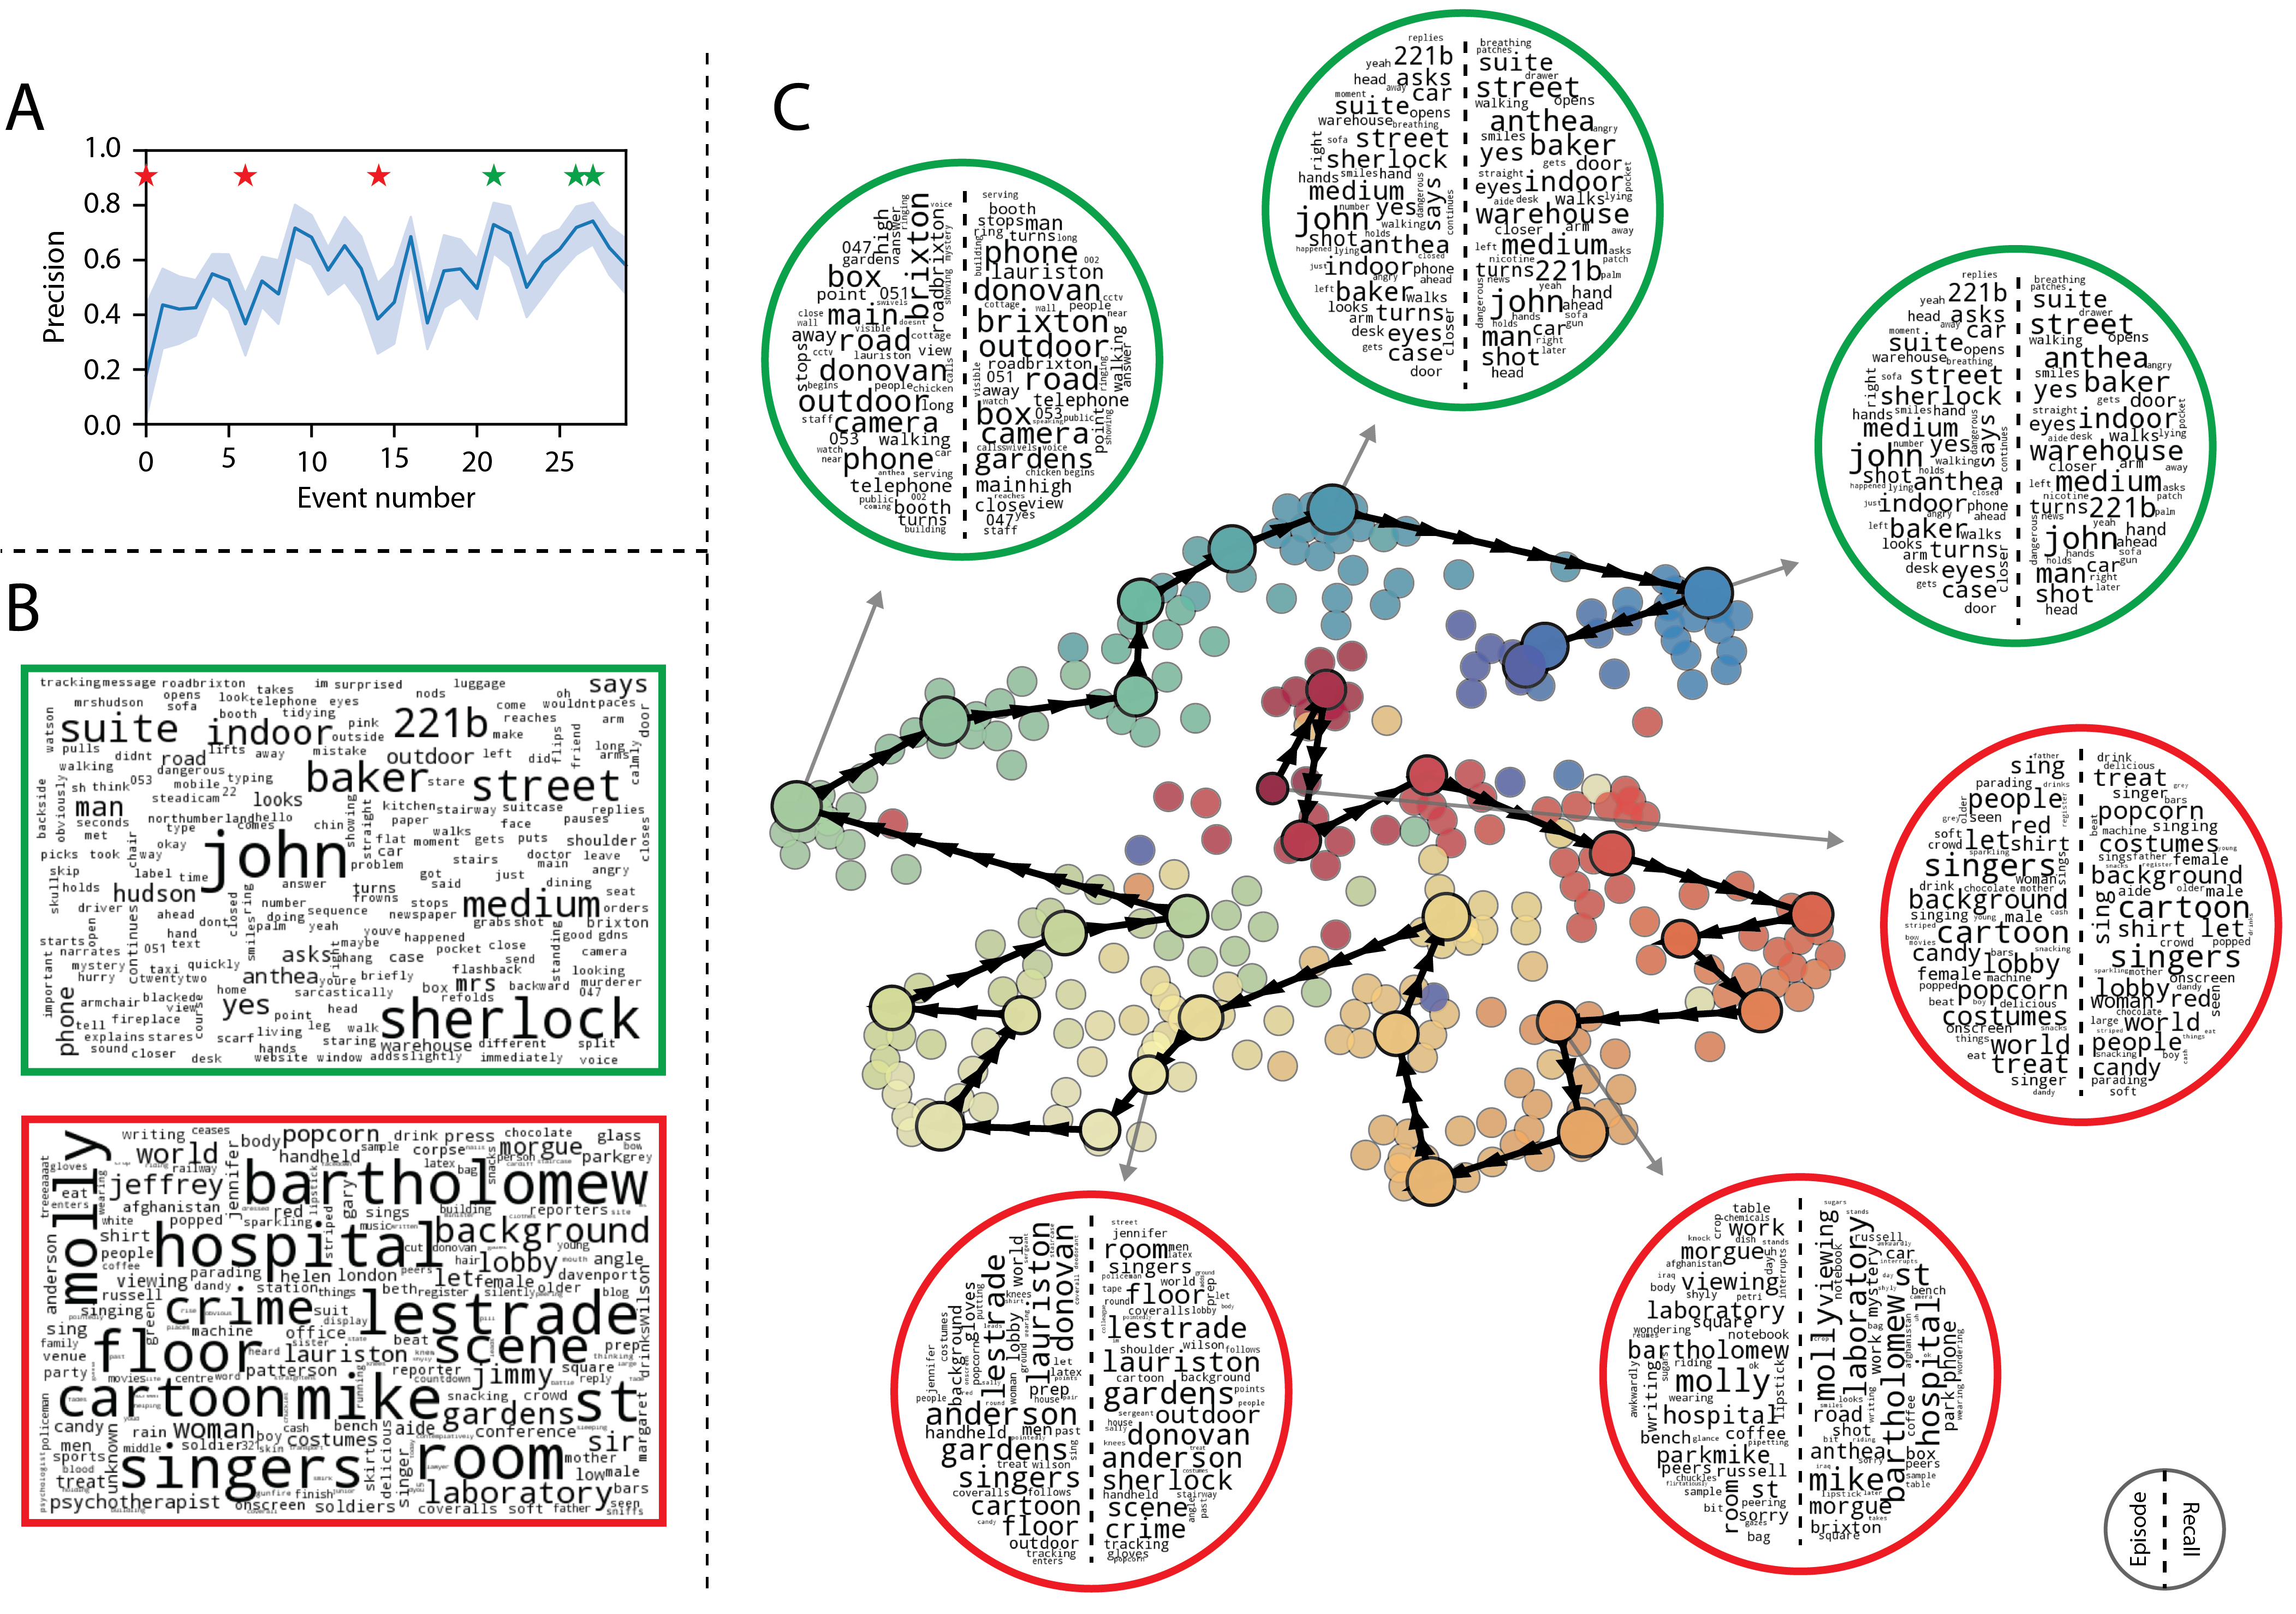
\includegraphics[width=1\textwidth]{figs/topics}
\caption{\small \textbf{Language used in the most and least memorable events.} \textbf{A.} Average precision (episode event-recall event topic vector correlation) across participants for each episode event.  Error bars denote bootstrap-derived across-participant 95\% confidence intervals.  The stars denote the three best-remembered events (green) and worst-remembered events (red).  \textbf{B.} Wordles comprising the top 200 highest-weighted words reflected in the weighted-average topic vector across episode events.  Green: episode events were weighted by how well the topic vectors derived from recalls of those events matched the episode events' topic vectors (Panel A).  Red: episode events were weighted by the inverse of how well their topic vectors matched the recalled topic vectors.  \textbf{C.}  The set of all episode and recall events is projected onto the two-dimensional space derived in Figure~\ref{fig:trajectory}.  The dots outlined in black denote episode events (dot size reflects the average correlation between the episode event's topic vector and the topic vectors from the closest matching recalled events from each participant; bigger dots denote stronger correlations).  The dots without black outlines denote recalled events.  All dots are colored using the same scheme as Figure~\ref{fig:trajectory}A.  Wordles for several example events are displayed (green: three best-remembered events; red: three worst-remembered events).  Within each circular wordle, the left side displays words associated with the topic vector for the episode event, and the right side displays words associated with the (average) recall event topic vector, across all recall events matched to the given episode event.}
\label{fig:topics}
\end{figure}

A similar result emerged from assessing the topic vectors for individual episode and recall events (Fig.~\ref{fig:topics}C).  Here, for each of the three best- and worst-remembered episode events, we have constructed two wordles: one from the original episode event's topic vector (left) and a second from the average recall topic vector for that event (right).  The three best-remembered events (circled in green) correspond to scenes integral to the central plot-line: a mysterious figure spying on John in a phone booth; John meeting Sherlock at Baker St. to discuss the murders; and Sherlock laying a trap to catch the killer.  Meanwhile, the three worst-remembered events (circled in red) reflect scenes that are non-essential to summarizing the narrative's structure: the video of singing cartoon characters participants viewed in an introductory clip prior to the main episode; John asking Molly about Sherlock's habit of over-analyzing people; and Sherlock noticing evidence of Anderson's and Donovan's affair.

The results thus far inform us about which aspects of the dynamic content in the episode participants watched were preserved or altered in participants' memories.  We next carried out a series of analyses aimed at understanding which brain structures might facilitate these preservations and transformations between the external world and memory.  In the first analysis, we sought to identify brain structures that were sensitive to the dynamic unfolding of the episode's content, as characterized by its topic trajectory.  We used a searchlight procedure to identify clusters of voxels whose activity patterns displayed a proximal temporal correlation structure (as participants watched the episode) matching that of the original episode's topic proportions (Fig.~\ref{fig:brainz}A; see \textit{Methods} for additional details).  In a second analysis, we sought to identify brain structures whose responses (during episode viewing) reflected how each participant would later structure their recounting of the episode.  We used an analogous searchlight procedure to identify clusters of voxels whose proximal temporal correlation matrices matched that of the topic proportions for each individual's recall (Figs.~\ref{fig:brainz}B; see \textit{Methods} for additional details).  To ensure our searchlight procedure identified regions \textit{specifically} sensitive to the temporal structure of the episode or recalls (i.e., rather than those with a temporal autocorrelation length similar to that of the episode/recalls), we performed a phase shift-based permutation correction (see \textit{Methods} for additional details). As shown in Figure~\ref{fig:brainz}C, the episode-driven searchlight analysis revealed a distributed network of regions that may play a role in processing information relevant to the narrative structure of the episode.  Similarly, the recall-driven searchlight analysis revealed a second network of regions (Fig.~\ref{fig:brainz}D) that may facilitate a person-specific transformation of one's experience into memory.  In identifying regions whose responses to ongoing experiences reflect how those experiences will be remembered later, this latter analysis extends classic \textit{subsequent memory analyses}~\citep[e.g.,][]{PallWagn02} to domain of naturalistic stimuli.

\begin{figure}[t]
\centering
\includegraphics[width=1\textwidth]{figs/searchlights}
\caption{\small \textbf{Brain structures that underlie the transformation of experience into memory.} \textbf{A.} We isolated the proximal diagonals from the upper triangle of the episode correlation matrix, and applied this same diagonal mask to the voxel response correlation matrix for each cube of voxels in the brain. We then searched for brain regions whose activation timeseries consistently exhibited a similar proximal correlational structure to the episode model, across participants.  \textbf{B.} We used dynamic time warping \citep{BernClif94} to align each participant's recall timeseries to the TR timeseries of the episode.  We then applied the same diagonal mask used in Panel A to isolate the proximal temporal correlations and searched for brain regions whose activation timeseries for an individual consistently exhibited a similar proximal correlational structure to each individual's recall.  \textbf{C.} We identified a network of regions sensitive to the narrative structure of participants' ongoing experience.  The map shown is thresholded at at $p < 0.05$, corrected.  \textbf{D}. We also identified a network or regions sensitive to how individuals would later structure the episode's content in their recalls.  The map shown is thresholded at at $p < 0.05$, corrected.}
\label{fig:brainz}
\end{figure}

The searchlight analyses described above yielded two distributed networks of brain regions, whose activity timecourses mirrored to the temporal structure of the episode (Fig.~\ref{fig:brainz}C) or participants' eventual recalls (Fig.~\ref{fig:brainz}D).  We next sought to gain greater insight into the structures and functional networks our results reflected.  To accomplish this, we performed an additional, exploratory analysis using \texttt{Neurosynth} \citep{YarkEtal11}.  Given an arbitrary statistical map as input, \texttt{Neurosynth} performs a massive automated meta-analysis, returning a ranked list of terms reported in papers with similar significance maps. We ran \texttt{Neurosynth} on the significance maps for the episode- and recall-driven searchlight analyses. These maps, along with the 10 terms with maximally similar meta-analysis images identified by \texttt{Neurosynth} are shown in Figure \ref{fig:neurosynth}.

\begin{figure}[t]
\centering
\includegraphics[width=1\textwidth]{figs/neurosynth_decoding}
\caption{\small \textbf{Decoding distributed statistical maps via Neurosynth meta-analyses.} \textbf{A.} episode-searchlight significance and top 10 decoded terms.  We constructed a map of the permutation-derived $p$-values for the episode-driven searchlight analysis (Fig.~\ref{fig:brainz}A, C) at each voxel with a positive permutation-derived $z$-score.  The top 10 terms decoded from this significance map are shown in red.  \textbf{B.} Recall-searchlight significance and top 10 decoded terms.  We constructed a map of the permutation-derived $p$-values for the recall-driven searchlight analysis (Fig.~\ref{fig:brainz}A, C) at each voxel with a positive permutation-derived $z$-score.  The top 10 terms decoded from this significance map are shown in blue.}
\label{fig:neurosynth}
\end{figure}
\FloatBarrier


\section*{Discussion}
\label{sec:discussion}

Our work casts remembering as reproducing (behaviorally and neurally) the topic trajectory, or shape, of an experience.  This view draws inspiration from prior work aimed at elucidating the neural and behavioral underpinnings of how we process dynamic naturalistic experiences and remember them later.  One approach to identifying neural responses to naturalistic stimuli (including experiences) entails building a model of the stimulus and searching for brain regions whose responses are consistent with the model.  In prior work, a series of studies from Uri Hasson's group~\citep{LernEtal11, SimoEtal16, ChenEtal17, BaldEtal17, ZadbEtal17} have extended this approach with a clever twist: rather than building an explicit stimulus model, these studies instead search for brain responses (while experiencing the stimulus) that are reliably similar across individuals.  So called \textit{inter-subject correlation} (ISC) and \textit{inter-subject functional connectivity} (ISFC) analyses effectively treat other people's brain responses to the stimulus as a ``model'' of how its features change over time.  By contrast, in our present work, we use topic models to construct an explicit content model directly from the stimulus (i.e., the topic trajectory of the episode).  Projecting each participant's recall into a space shared by both the stimulus and other participants then allows us to compare recalls both directly to the stimulus and to each other.  Similarly, prior work introducing the use of HMMs to discover latent event structure in naturalistic stimuli and recall \citep{BaldEtal17} used between-subjects cross-validation to identify event boundaries shared across participants, and between stimulus and recall.  Our framework allows us to break from the restriction of a common, shared event-timeseries and identify the unique \textit{resolution} of each participant's recall event structure, and how that may differ from the episode and that of other participants.
% @JEREMY @ANDY PLEASE CHECK THIS TO MAKE SURE I'M NOT MISCHARACTERIZING BALDETAL17

Word embedding models are a rapidly growing area of machine learning research.  Early approaches including latent
  semantic analysis~\citep{LandDuma97} use word co-occurrence statistics (i.e., how often pairs of words occur in the same documents contained in the corpus) to derive a unique feature vector for each word.  The feature vectors are constructed so that words that co-occur more frequently have feature vectors that are closer (in Euclidean distance).  Related approaches, such as latent dirichlet
  allocation~\citep{BleiEtal03} attempt to explicitly model the underlying causes of word co-occurrences by automatically identifying the set of themes or topics reflected across the documents in the corpus.  More recent work on these types of semantic models, including word2vec~\citep{MikoEtal13}, the Universal Sentence Encoder~\citep{CerEtal18}, GPT-2~\citep{RadfEtal19}, and GTP-3~\citep{BrowEtal20} use deep neural networks to attempt to identify the deeper conceptual representations underlying each word.  Despite the growing popularity of more sophisticated deep learning-based embedding models, here we leverage latent dirichlet allocation (i.e., topic modeling) to embed episode and recall text.  This decision was motivated by several factors.  First, topic models capture the \textit{essence} of a text passage devoid of the specific set and order of words used.  This was an important feature of our model since different people may accurately recall a scene using very different language. Second, words can mean different things in different contexts (e.g. ``bat'' may be the act of hitting a baseball, the object used for that action, or as a flying mammal).  Topic models are robust to this, allowing words to exist as part of multiple topics.  Last, topic models provide a straightforward means of recovering the weights for the particular words comprising a topic, enabling straightforward interpretation of an event's contents (e.g. Fig.~\ref{fig:topics}). Other models such as the Universal Sentence Encoder, GPT-2, and GPT-3 offer context-sensitive encoding of text passages, but the encoding space is complex and non-linear, and thus recovering the original words used to fit the model is not straightforward. However, it is worth pointing out that our general framework is divorced from the particular choice of language model. Moreover, many of the aspects of our framework could be swapped out for other choices. For example, the language model, the timeseries segmentation model and the episode-recall matching function could all be customized to suit a particular question space or application. Indeed for some questions, recovery of the particular words used to describe a memory may not be necessary, and thus other text-modeling approaches (including the deep learning-based embedding models described above) may be preferable. Future work will explore the influence of particular model choices on the framework's efficacy.

In extending classical free recall analyses to our naturalistic memory framework, we recovered two patterns of recall dynamics central to list-learning studies: a heightened probability of initiating recall with the first presented ``item" (in our case, episode events; Fig.~\ref{fig:list-learning}A) and a strong bias toward transitioning from recalling a given event to recalling the one immediately following it (Fig.~\ref{fig:list-learning}B).  However, equally noteworthy are the typical free recall results \textit{not} recovered in these analyses, as each highlights a fundamental difference between the list-learning paradigm and naturalistic memory paradigms like the one employed in the present study.  The most noticeable departure from hallmark free recall dynamics in these findings is the apparent lack of a serial position effect in Figure \ref{fig:list-learning}C, which instead shows greater and lesser recall probabilities for events distributed across the episode.  Stimuli in free recall experiments most often comprise lists of simple, common words, presented to participants in a random order. \citep[In fact, numerous word pools have been developed based on these criteria; e.g.,][]{FrieEtal82}.  These stimulus qualities enable two assumptions that are central to word list analyses, but frequently do not hold for real-world experiences.  First, researchers conducting list-learning studies may assume that the content at each presentation index is essentially equal, and does not possess attributes that would render it, on average, more or less memorable than others.  Such is rarely the case with real-world experiences or experiments meant to approximate them, and the effects of both intrinsic and observer-dependent factors on stimulus memorability are well established \citep[for review see][]{ChunTurk07, ByliEtal15, TyngEtal17}.  Second, the random ordering of list items ensures that (across participants, on average) there is no relationship between the thematic similarity of individual stimuli and their presentation positions---in other words, two successively presented items are no more likely to be highly semantically similar than they are to be highly dissimilar.  In most cases, the exact opposite is true of real-world episodes.  Our internal thoughts, our actions, and the physical state of the world around us all tend to follow a direct (often causal) progression.  As a result, each moment of our experience tends to be inherently more similar to surrounding moments than to those in the distant past or future.  Memory literature has termed this strong temporal autocorrelation ``context," and in various media that depict real-world events (e.g., movies or written stories), we recognize it as a \textit{narrative structure}.  While a random word list (by definition) has no such structure, the logical progression between ideas and actions in a naturalistic stimulus prompts the rememberer to recount presented events in order, starting with the beginning.  This tendency is reflected in our findings' second departure from typical free recall dynamics: a lack of increased probability of first recall for end-of-sequence events (Fig.~\ref{fig:list-learning}A).

Because they disregard presentation order-dependent variability in the stimulus content, analyses such as those in Figure \ref{fig:list-learning} enable a more sensitive analysis of presentation order-dependent temporal dynamics in free recall. Yet by the same token, they paint a wholly incomplete picture of memory for naturalistic episodes.  In an attempt to address this shortcoming, we have developed a framework in the present study that characterizes the explicit semantic content of the stimulus and subsequent recalls.  However, sensitivity to stimulus and recall content introduces a new challenge: distinguishing between levels of recall quality for a stimulus (e.g., an event) that is considered to have been ``remembered."  When modeling memory in an experimental setting, recall quality for individual events is often cast as binary (e.g., a given list item was simply either remembered or not remembered).  Various models of memory (e.g., \citealp{Yone02}) attempt to improve upon this by including confidence ratings, rendering this binary judgement instead categorical.  To better evaluate naturalistic memory quality, we introduce a continuous metric (\textit{precision}), which reflects the level of completeness of a participant's recall for a feature-rich experience.  Additionally, recall quality for a single event is typically assessed independently from that for all other events (e.g., it is difficult to ``compare" a participant's binary recall success for list item 1 to that of list item 10).  The second novel metric we introduce (\textit{distinctiveness}) is based on analyzing of the correlational structure of an individual's full set of recall events, and reflects the specificity of their memory for a single experienced event.  We find that both of these metrics relate to the overall number of episode events participants successfully recalled, and that our precision metric additionally relates to \cite{ChenEtal17}'s hand-annotated memory memory scores.

We did not find evidence that participants' average recall distinctiveness was related to their hand-annotated memory scores computed by~\cite{ChenEtal17}.  One possible explanation is that, in hand-scoring each participant's verbal recall for each of 50 (manually-deliniated) scenes, ``[a] scene was counted as recalled if the participant described any part of the scene''~\citep{ChenEtal17}.  In other words, both an extensive description of a scene's content and a brief mention of some subset of its content were (binarily) considered equally successful recalls.  By contrast, we identify the event structure in participants' recalls in an unsupervised manner, independent of the episode event-timeseries, prior to mapping between episode and recall content.  Our HMM-based event-segmentation produces boundaries between timepoints where the topic proportions shift in a substantial way, and because a small handful of words is unlikely to contribute significantly to the topic proportions for any sliding window, such brief scene descriptions will most often not result in a sufficiently large shift in the resulting topic proportions for the HMM to identify an event boundary.  Instead, they will be grouped with a neighboring event, consequently lowering that event's distinctiveness score and by extension, the participant's overall distinctiveness score.  This is in essence the qualitative difference between distinctive and indistinctive recall, and reflects the comparison shown in Figure \ref{fig:distinctiveness-detail}C.  Intriguingly, prior studies show that pattern separation, or the ability to cleanly discriminate between similar experiences, is impaired in many cognitive disorders as well as natural aging \citep{StarEtal10, YassEtal11c, YassStar11b}.  Future work might explore whether and how these metrics compare between cognitively impoverished groups and healthy controls.

In the analyses outlined in Figure \ref{fig:brainz}, we identified two networks of brain regions whose responses during episode viewing were consistent with the temporal structure of the episode and recall topic trajectories, respectively. The network identified by the episode trajectory analysis included the ventromedial prefrontal cortex, left anterior temporal lobe, superior parietal and dorsal anterior cingulate cortex. The network from the episode-recall trajectory analysis also included the ventromedial prefrontal and superior parietal cortices, in addition to the posterior medial cortex (PMC) and the inferior temporal regions. Notably, \cite{ChenEtal17} also observed the PMC in a number of analyses including one that searched for regions whose activity patterns during encoding were reinstated during free recall. The PMC has been consistently identified in studies involving stimuli with meaningfully structured events~\citep{CohnRang17}. Further, the PMC is part of the "posterior medial" system, a network of brain regions thought to represent situation models~\citep{ZackEtal07} in support of memory, spatial navigation and social cognition~\citep{RangRitc12}. Given that we constructed our episode-recall searchlight model to capture temporal structure in the episode's semantic content (and how one's later recall aligns with that structure), we speculate that the PMC may play a role in constructing mnemonic events from meaningfully structured experiences.

Decoding the associated significance maps with \texttt{Neurosynth} revealed two intriguing results.  First, the top 10 terms returned for the episode-driven searchlight significance map were centered around themes of language and semantic meaning (Fig.~\ref{fig:neurosynth}A).  In other words, the voxels identified as more reflective of the episode content's temporal structure (i.e., voxels with lower permutation correction-derived $p$-values), as defined by our model, were most likely to be reported as active in studies focused on the the neural underpinnings of semantic processing.  This finding is interesting, as our model specifically captures the temporal structure of the episode's \textit{semantic} content (e.g., as opposed to that of the visual, auditory, or affective content).  This suggests that the network of structures displayed in Figure \ref{fig:brainz}C may play a roll in processing the evolving semantic content of ongoing experiences.


Our second searchlight analysis identified a partially overlapping network of regions (Fig.~\ref{fig:brainz}D) whose patterns of activity as participants viewed the episode reflected the idiosyncratic structure of each individual's later recalls.  The associated significance map yielded a set of \texttt{Neurosynth} terms that primarily reflected names of specific structural regions (such as ``thalamus," ``anterior insula," ``anterior cingulate" and ``inferior frontal"; Fig.~\ref{fig:neurosynth}B).  Interestingly, these regions share membership in a common, large-scale functional network (termed the ``salience network") involved in detecting and processing affective cues.  In particular, the latter three regions have been implicated in functions relevant to assigning personal meaning to an experience, including: ascribing subjective value to raw, sensory input \citep{MedfCrit10}; modulating semantic and phonological processing in response to personally salient stimuli \citep{KellEtal07b}; and directing and reallocating attention and working memory resources towards the most relevant stimuli \citep{MenoUddi10}.  This suggests that the network of structures displayed in Figure \ref{fig:brainz}D may be play a roll in transforming and restructuring ongoing experiences through the lens of one's prior experience and subjective emotions as they are encoded in memory.

Our work has broad implications for how we characterize and assess memory in real-world settings, such as the classroom or physician's office.  For example, the most commonly used classroom evaluation tools involve simply computing the proportion of correctly answered exam questions.  Our work indicates that this approach is only loosely related to what educators might really want to measure: how well did the students understand the key ideas presented in the course?  Under this typical framework of assessment, the same exam score of 50\% could be ascribed to two very different students: one who attended the full course but struggled to learn more than a broad overview of the material, and one who attended only half of the course but understood the material perfectly.  Instead, one could apply our computational framework to build explicit content models of the course material and exam questions.  This approach would provide a more nuanced and specific view into which aspects of the material students had learned well (or poorly).  In clinical settings, memory measures that incorporate such explicit content models might also provide more direct evaluations of patients' memories.


\section*{Methods}
\label{sec:methods}

\subsection*{Experimental design and data collection}
Data were collected by \cite{ChenEtal17}.  In brief, participants ($n=22$) viewed the first 48 minutes of ``A Study in Pink'', the first episode of the BBC television series \textit{Sherlock}, while fMRI volumes were collected (TR = 1500~ms).  Participants were pre-screened to ensure they had never seen any episode of the show before.  The stimulus was divided into a 23~min (946~TR) and a 25~min (1030~TR) segment to mitigate technical issues related to the scanner.  After finishing the clip, participants were instructed to \citep[quoting from][]{ChenEtal17} ``describe what they recalled of the [episode] in as much detail as they could, to try to recount events in the original order they were viewed in, and to speak for at least 10 minutes if possible but that longer was better. They were told that completeness and detail were more important than temporal order, and that if at any point they realized they had missed something, to return to it. Participants were then allowed to speak for as long as they wished, and verbally indicated when they were finished (e.g., `I’m done').''  Five participants were dropped from the original dataset due to excessive head motion (2 participants), insufficient recall length (2 participants), or falling asleep during stimulus viewing (1 participant), resulting in a final sample size of $n=17$.  For additional details about the experimental procedure and scanning parameters, see \cite{ChenEtal17}.  The experimental protocol was approved by Princeton University's Institutional Review Board.

After preprocessing the fMRI data and warping the images into a standard (3~mm$^3$ MNI) space, the voxel activations were $z$-scored (within voxel) and spatially smoothed using a 6~mm (full width at half maximum) Gaussian kernel.  The fMRI data were also cropped so that all episode-viewing data were aligned across participants.  This included a constant 3 TR (4.5~s) shift to account for the lag in the hemodynamic response.  \citep[All of these preprocessing steps followed][where additional details may be found.]{ChenEtal17}

The video stimulus was divided into 1,000 fine-grained ``scenes" and annotated by an independent coder.  For each of these 1,000 scenes, the following information was recorded: a brief narrative description of what was happening, the location where the scene took place, whether that location was indoors or outdoors, the names of all characters on-screen, the name(s) of the character(s) in focus in the shot, the name(s) of the character(s) currently speaking, the camera angle of the shot, a transcription of any text appearing on-screen, and whether or not there was music present in the background.  Each scene was also tagged with its onset and offset time, in both seconds and TRs.

\subsection*{Data and code availability}
The fMRI data we analyzed are available online \href{http://dataspace.princeton.edu/jspui/handle/88435/dsp01nz8062179}{\underline{here}}.  The behavioral data and all of our analysis code may be downloaded \href{https://github.com/ContextLab/sherlock-topic-model-paper}{\underline{here}}.

\subsection*{Statistics}
All statistical tests performed in the behavioral analyses were two-sided.  All statistical tests performed in the neural data analyses were two-sided, except for the permutation-based thresholding, which was one-sided.  In this case, we were specifically interested in identifying voxels whose activation time series reflected the temporal structure of the episode and recall trajectories to a \textit{greater} extent than that of the phase-shifted trajectories.
% ------ NOTE: ------
% from the Nature Human Behavior submission requirements: "Specify whether tests were one- or two-tailed, and justify the use of one-tailed tests."
% - Paxton

\subsection*{Modeling the dynamic content of the episode and recall transcripts}
\subsubsection*{Topic modeling}
The input to the topic model we trained to characterize the dynamic content of the episode comprised 998 hand-generated annotations of short (mean: 2.96s) scenes spanning the video clip~(\citealp{ChenEtal17} generated 1000 annotations total; we removed two annotations referring to a break between the first and second scan sessions, during which no fMRI data was collected).  We concatenated the text for all of the annotated features within each segment, creating a ``bag of words'' describing each scene and performed some minor preprocessing (e.g., stemming possessive nouns and removing punctuation).  We then re-organized the text descriptions into overlapping sliding windows spanning (up to) 50 scenes each.  In other words, we estimated the ``context'' for each scene using the text descriptions of the preceding 25 scenes, the present scene, and the following 24 scenes.  To model the context for scenes near the beginning of the episode (i.e., within 25 scenes of the beginning or end), we created overlapping sliding windows that grew in size from one scene to the full length.  We also tapered the sliding window lengths at the end of the episode, whereby scenes within fewer than 24 scenes of the end of the episode were assigned sliding windows that extended to the end of the episode.  This procedure ensured that each scene's content was represented in the text corpus an equal number of times.
% ------ NOTE: ------
% need to refine explanation here a little bit
% - Paxton

We trained our model using these overlapping text samples with \texttt{scikit-learn}~\citep[version 0.19.1; ][]{PedrEtal11}, called from our high-dimensional visualization and text analysis software, \texttt{HyperTools}~\citep{HeusEtal18a}.  Specifically, we used the \texttt{CountVectorizer} class to transform the text from each window into a vector of word counts (using the union of all words across all scenes as the ``vocabulary,'' excluding English stop words); this yielded a number-of-windows by number-of-words \textit{word count} matrix.  We then used the \texttt{LatentDirichletAllocation} class (topics=100, method=`batch') to fit a topic model~\citep{BleiEtal03} to the word count matrix, yielding a number-of-windows (1047) by number-of-topics (100) \textit{topic proportions} matrix.  The topic proportions matrix describes the gradually evolving mix of topics (latent themes) present in each scene.  Next, we transformed the topic proportions matrix to match the 1976 fMRI volume acquisition times.  We assigned each topic vector to the timepoint (in seconds) midway between the beginning of the first scene and the end of the last scene in its corresponding sliding text window.  By doing so, we warped the linear temporal distance between consecutive topic vectors to align with the inconsistent temporal distance between consecutive annotations (whose durations varied greatly).  We then rescaled these timepoints to 1.5s TR units, and used linear interpolation to estimate a topic vector for each TR.  This resulted in a number-of-TRs (1976) by number-of-topics (100) matrix.

We created similar topic proportions matrices using hand-annotated transcripts of each participant's verbal recall of the episode~\citep[annotated by][]{ChenEtal17}.  We tokenized the transcript into a list of sentences, and then re-organized the list into overlapping sliding windows spanning (up to) 10 sentences each, analogously to how we parsed the episode annotations.  In turn, we transformed each window's sentences into a word count vector (using the same vocabulary as for the episode model), and then we used the topic model already trained on the episode scenes to compute the most probable topic proportions for each sliding window.  This yielded a number-of-windows (range: 83--312) by number-of-topics (100) topic proportions matrix for each participant.  These reflected the dynamic content of each participant's recalls.  Note: for details on how we selected the episode and recall window lengths and number of topics, see \textit{Supporting Information} and Figure~\topicopt.


\subsubsection*{Parsing topic trajectories into events using Hidden Markov Models}
We parsed the topic trajectories of the episode and participants' recalls into events using Hidden Markov Models~\citep[HMMs;][]{Rabi89}.  Given the topic proportions matrix (describing the mix of topics at each timepoint) and a number of states, $K$, an HMM recovers the set of state transitions that segments the timeseries into $K$ discrete states.  Following \cite{BaldEtal17}, we imposed an additional set of constraints on the discovered state transitions that ensured that each state was encountered exactly once (i.e., never repeated).  We used the BrainIAK toolbox~\citep{Brainiak} to implement this segmentation.

We used an optimization procedure to select the appropriate $K$ for each topic proportions matrix.  Prior studies on narrative structure and processing have shown that we both perceive and internally represent the world around us at multiple, hierarchical timescales \citep[e.g.,][]{HassEtal08, LernEtal11, HassEtal15, ChenEtal17, BaldEtal17, BaldEtal18}.  However, for the purposes of our framework, we sought to identify the single timeseries of event-representations that is emphasized \textit{most heavily} in the temporal structure of the episode and of each participant's recall.  We quantified this as the set of $K$ states that maximized the similarity between topic vectors for timepoints comprising each state, while minimizing the similarity between topic vectors for timepoints across different states.  Specifically, we computed (for each matrix)
\[
  \argmax_K \left[W_{1}(a, b)\right],
\]
where $a$ was the distribution of within-state topic vector correlations, and $b$ was the distribution of across-state topic vector correlations .  We computed the first Wasserstein distance ($W_{1}$; also known as \textit{Earth mover's distance}; \citealp{Dobr70, RamdEtal17}) between these distributions for a large range of possible $K$-values (range [2, 50]), and selected the $K$ that yielded the maximum value.  Figure~\ref{fig:model}B displays the event boundaries returned for the episode, and Figure~\corrmats~displays the event boundaries returned for each participant's recalls.  See Figure \kopt~for the optimization functions for the episode and recalls.  After obtaining these event boundaries, we created stable estimates of the content represented in each event by averaging the topic vectors across timepoints between each pair of event boundaries.  This yielded a number-of-events by number-of-topics matrix for the episode and recalls from each participant.

\subsubsection*{Naturalistic extensions of classic list-learning analyses}
In traditional list-learning experiments, participants view a list of items (e.g., words) and then recall the items later.  Our episode-recall event matching approach affords us the ability to analyze memory in a similar way. The episode and recall events can be treated analogously to studied and recalled ``items'' in a list-learning study.  We can then extend classic analyses of memory performance and dynamics (originally designed for list-learning experiments) to the more naturalistic episode recall task used in this study.

Perhaps the simplest and most widely used measure of memory performance is \textit{accuracy}---i.e., the proportion of studied (experienced) items (in this case, episode events) that the participant later remembered.  \cite{ChenEtal17} used this method to rate each participant's memory quality by computing the proportion of (50, manually identified) scenes mentioned in their recall.  We found a strong across-participants correlation between these independent ratings and the proportion of 30 HMM-identified episode events matched to participants' recalls (Pearson's $r(15) = 0.71, p = 0.002$).  We further considered a number of more nuanced memory performance measures that are typically associated with list-learning studies.  We also provide a software package, \texttt{Quail}, for carrying out these analyses~\citep{HeusEtal17b}.

\paragraph{Probability of first recall (PFR).}  PFR curves~\citep{WelcBurn24, PostPhil65, AtkiShif68} reflect the probability that an item will be recalled first as a function of its serial position during encoding. To carry out this analysis, we initialized a number-of-participants (17) by number-of-episode-events (30) matrix of zeros. Then for each participant, we found the index of the episode event that was recalled first (i.e., the episode event whose topic vector was most strongly correlated with that of the first recall event) and filled in that index in the matrix with a 1.  Finally, we averaged over the rows of the matrix, resulting in a 1 by 30 array representing the proportion of participants that recalled an event first, as a function of the order of the event's appearance in the episode (Fig.~\ref{fig:list-learning}A).
% ------ NOTE: ------
% reiterate meaning of error ribbons in list-learning figure? (already noted in figure caption)
% - Paxton

\paragraph{Lag conditional probability curve (lag-CRP).} The lag-CRP curve~\citep{Kaha96} reflects the probability of recalling a given item after the just-recalled item, as a function of their relative encoding positions (or \textit{lag}).  In other words, a lag of 1 indicates that a recalled item was presented immediately after the previously recalled item, and a lag of -3 indicates that a recalled item came 3 items before the previously recalled item.  For each recall transition (following the first recall), we computed the lag between the current recall event and the next recall event, normalizing by the total number of possible transitions.  This yielded a number-of-participants (17) by number-of-lags (-29 to +29; 58 lags total excluding lags of 0) matrix. We averaged over the rows of this matrix to obtain a group-averaged lag-CRP curve (Fig.~\ref{fig:list-learning}B).

\paragraph{Serial position curve (SPC).} SPCs~\citep{Murd62a} reflect the proportion of participants that remember each item as a function of the items' serial positions during encoding. We initialized a number-of-participants (17) by number-of-episode-events (30) matrix of zeros. Then, for each recalled event, for each participant, we found the index of the episode event that the recalled event most closely matched (via the correlation between the events' topic vectors) and entered a 1 into that position in the matrix. This resulted in a matrix whose entries indicated whether or not each event was recalled by each participant (depending on whether the corresponding entires were set to one or zero).  Finally, we averaged over the rows of the matrix to yield a 1 by 30 array representing the proportion of participants that recalled each event as a function of the events' order appearance in the episode (Fig.~\ref{fig:list-learning}C).

\paragraph{Temporal clustering scores.} Temporal clustering describes a participant's tendency to organize their recall sequences by the learned items' encoding positions.  For instance, if a participant recalled the episode events in the exact order they occurred (or in exact reverse order), this would yield a score of 1.  If a participant recalled the events in random order, this would yield an expected score of 0.5.  For each recall event transition (and separately for each participant), we sorted all not-yet-recalled events according to their absolute lag (i.e., distance away in the episode).  We then computed the percentile rank of the next event the participant recalled.  We averaged these percentile ranks across all of the participant's recalls to obtain a single temporal clustering score for the participant.

\paragraph{Semantic clustering scores.} Semantic clustering describes a participant's tendency to recall semantically similar presented items together in their recall sequences.  Here, we used the topic vectors for each event as a proxy for its semantic content. Thus, the similarity between the semantic content for two events can be computed by correlating their respective topic vectors.  For each recall event transition, we sorted all not-yet-recalled events according to how correlated the topic vector \textit{of the closest-matching episode event} was to the topic vector of the closest-matching episode event to the just-recalled event.  We then computed the percentile rank of the observed next recall.  We averaged these percentile ranks across all of the participant's recalls to obtain a single semantic clustering score for the participant.

% To quantify the similarity between the episode topic trajectory and individual recall topic trajectories, we considered several novel metrics.  First, we tested whether each participant's recall trajectory matched the episode trajectory in a general sense. For each participant, we filtered the episode trajectory to only include the events that the participant remembered.  We then computed the root mean squared difference (RMSD) between the remaining episode events and the (closest-matching) recalled events.  For example, if the topic vectors for a participant's recall event topic vectors matched the corresponding episode event topic vectors exactly (and in order), the expected RMSD for those events would be 0.  However, if the participant's recall events did not perfectly match the episode events, or if they were out of order, then the RMSD would be greater than 0.  To assess the significance of the match between the episode and recall trajectories, we carried out a permutation procedure whereby, for each of 10000 repetitions, we circularly shifted the recall trajectories (in time) by a random amount and then re-computed the RMSD each time.  This yielded a distribution of ``null'' RMSD values for each participant.  The observed RMSD values reached significance (i.e., $p < 0.05$, reflecting that more than 95\% of the null RMSD values were greater than the observed RMSD value) for nine of the participants (3, 4, 8--13, and 17).  (For the remaining participants this test yielded $0.05 \leq p < 0.25$.)  The observed RMSD values were also reliably correlated with hand-annotated memory performance across participants (Pearson's $r(15) = -0.57, p = 0.016$).  In other words, a closer match between the episode and recall topic trajectories was related to better overall recall performance.
% ------ NOTE: ------
% Andy was thinking about including this in the revision early on.  It wasn't in the preprint version, and with how much else we have in here, I don't think it's worth including anymore.
% - Paxton
% I agree that we can take it out. -AH


\subsubsection*{Novel naturalistic memory metrics}

\paragraph*{Precision.}
We tested whether participants who recalled more events were also more \textit{precise} in their recollections. For each participant, we computed the average correlation between the topic vectors for each recall event and those of its closest-matching episode event. This gave a single value per participant representing the average precision across all recalled events.  We then correlated these values with both hand-annotated and model-derived (i.e., the number of unique episode events matched by a participant's recall events) memory performance.

\paragraph*{Distinctiveness.}
We also considered the \textit{distinctiveness} of each recalled event. That is, how unique a participant's description of a episode event was, versus their descriptions of other episode events.  We hypothesized that participants with high memory performance might describe each event in a more distinctive way (relative to those with lower memory performance who might describe events in a more general way).  To test this hypothesis we define a distinctiveness score for each recall event $i$ as

\[
  d(i) = 1 - \frac{1}{N - 1} \sum_{j = \\i}\mathrm{corr}\left(\mathrm{event}_i, \mathrm{event}_j\right) 
\]
where the average is taken over the correlation between the recall event $i$'s topic vector and the topic vectors from all other recall events from that participant.  We averaged these distinctiveness scores across all of the events recalled by the given participant to get the participant's distinctiveness score.  We correlated these distinctiveness scores with hand-annotated and model-derived memory performance scores across-subjects, as above.

\paragraph*{Averaging correlations}
In all instances where we performed statistical tests involving precision or distinctiveness scores, we used the Fisher $z$-transformation~\citep{Fish25} to stabilize the variance across the distribution of correlation values prior to performing the test.  Similarly, when averaging precision or distinctiveness scores, we $z$-transformed the scores prior to computing the mean, and inverse $z$-transformed the result.

\subsubsection*{Visualizing the episode and recall topic trajectories}
We used the UMAP algorithm~\citep{McInEtal18} to project the 100-dimensional topic space onto a two-dimensional space for visualization (Figs.~\ref{fig:trajectory}, \ref{fig:topics}).  To ensure that all of the trajectories were projected onto the \textit{same} lower dimensional space, we computed the low-dimensional embedding on a ``stacked'' matrix created by vertically concatenating the events-by-topics topic proportions matrices for the episode, across-participants average recall and all 17 individual participants' recalls.  We then separated the rows of the result (a total-number-of-events by two matrix) back into individual matrices for the episode topic trajectory, across-participant average recall trajectory and the trajectories for each individual participant's recalls (Fig.~\ref{fig:trajectory}).  This general approach for discovering a shared low-dimensional embedding for a collections of high-dimensional observations follows \cite{HeusEtal18a}.

We optimized the manifold space for visualization based on two criteria: First, that the 2D embedding of the episode trajectory should reflect its original 100-dimensional structure as faithfully as possible. Second, that the path traversed by the embedded episode trajectory should intersect itself a minimal number of times.  The first criteria helps bolster the validity of visual intuitions about relationships between sections of episode content, based on their locations in the embedding space.  The second criteria was motivated by the observed low off-diagonal values in the episode trajectory's temporal correlation matrix (suggesting that the same topic-space coordinates should not be revisited; see Figure~2A in the main text). For further details on how we created this low-dimensional embedding space, see \textit{Supporting Information}.

\subsubsection*{Estimating the consistency of flow through topic space across participants}
In Figure~\ref{fig:trajectory}B, we present an analysis aimed at characterizing locations in topic space that different participants move through in a consistent way (via their recall topic trajectories).  The two-dimensional topic space used in our visualizations (Fig.~\ref{fig:trajectory}) comprised a 60 x 60 (arbitrary units) square.  We tiled this space with a 50 x 50 grid of evenly spaced vertices, and defined a circular area centered on each vertex whose radius was two times the distance between adjacent vertices (i.e., 2.4 units).  For each vertex, we examined the set of line segments formed by connecting each pair successively recalled events, across all participants, that passed through this circle.  We computed the distribution of angles formed by those segments and the $x$-axis, and used a Rayleigh test to determine whether the distribution of angles was reliably ``peaked'' (i.e., consistent across all transitions that passed through that local portion of topic space).  To create Figure~\ref{fig:trajectory}B we drew an arrow originating from each grid vertex, pointing in the direction of the average angle formed by the line segments that passed within 2.4 units.  We set the arrow lengths to be inversely proportional to the $p$-values of the Rayleigh tests at each vertex.  Specifically, for each vertex we converted all of the angles of segments that passed within 2.4 units to unit vectors, and we set the arrow lengths at each vertex proportional to the length of the (circular) mean vector.  We also indicated any significant results ($p < 0.05$, corrected using the Benjamani-Hochberg procedure) by coloring the arrows in blue (darker blue denotes a lower $p$-value, i.e., a longer mean vector); all tests with $p \geq 0.05$ are displayed in gray and given a lower opacity value.

\subsection*{Searchlight fMRI analyses}
In Figure~\ref{fig:brainz}, we present two analyses aimed at identifying brain regions whose responses (as participants viewed the episode) exhibited a particular temporal structure.  We developed a searchlight analysis wherein we constructed a 5 x 5 x 5 cube of voxels (following \citealp{ChenEtal17}) centered on each voxel in the brain, and for each of these cubes, computed the temporal correlation matrix of the voxel responses during episode viewing.  Specifically, for each of the 1976 volumes collected during episode viewing, we correlated the activity patterns in the given cube with the activity patterns (in the same cube) collected during every other timepoint.  This yielded a 1976 by 1976 correlation matrix for each cube.  Note: participant 5's scan ended 75s early, and in \citealp{ChenEtal17}'s publicly released dataset, their scan data was padded to match the length of the other participants'.  For our searchlight analyses, we removed this padded data (i.e., the last 50 TRs), resulting in a 1925 by 1925 correlation matrix for each cube in participant 5's brain.

Next, we constructed a series of ``template'' matrices.  The first template reflected the timecourse of the episode's topic trajectory, and the others reflected the timecourse of each participant's recall trajectory.  To construct the episode template, we computed the correlations between the topic proportions estimated for every pair of TRs (prior to segmenting the trajectory into discrete events; i.e., the correlation matrix shown in Figs.~\ref{fig:model}B and \ref{fig:brainz}A).  We constructed similar temporal correlation matrices for each participant's recall topic trajectory (Figs.~\ref{fig:model}D, \corrmats).  However, to correct for length differences and potential non-linear transformations between viewing time and recall time, we first used dynamic time warping~\citep{BernClif94} to temporally align participants' recall topic trajectories with the episode topic trajectory.  An example correlation matrix before and after warping is shown in Fig.~\ref{fig:brainz}B.  This yielded a 1976 by 1976 correlation matrix for the episode template and for each participant's recall template.

The temporal structure of the episode's content (as described by our model) is captured in the block-diagonal structure of the episode's temporal correlation matrix (e.g., Figs.~\ref{fig:model}B, \ref{fig:brainz}A), with time periods of thematic stability represented as dark blocks of varying sizes.  Inspecting the episode correlation matrix suggests that the episode's semantic content is highly temporally specific (i.e., the correlations between topic vectors from distant timepoints are almost all near zero).  By contrast, the activity patterns of individual (cubes of) voxels can encode relatively limited information on their own, and their activity frequently contributes to multiple separate functions \citep{FreeEtal01, SigmDeha08, CharKoec10, RishEtal13}.  By nature, these two attributes give rise to similarities in activity across large timescales that may not necessarily reflect a single task.  To enable a more sensitive analysis of brain regions whose shifts in activity patterns mirrored shifts in the semantic content of the episode or recalls, we restricted the temporal correlations we considered to the timescale of semantic information captured by our model.  Specifically, we isolated the upper triangle of the episode correlation matrix and created a ``proximal correlation mask'' that included only diagonals from the upper triangle of the episode correlation matrix up to the first diagonal that contained no positive correlations.  Applying this mask to the full episode correlation matrix was analogous to excluding diagonals beyond the corner of the largest diagonal block.  In other words, the timescale of temporal correlations we considered corresponded to the longest period of thematic stability in the episode, and by extension the longest expected period of thematic stability in participants' recalls and the longest period of stability we might expect to see in voxel activity arising from processing or encoding episode content.  Figure \ref{fig:brainz} shows this proximal correlation mask applied to the temporal correlation matrices for the episode, an example participant's (warped) recall, and an example cube of voxels from our searchlight analyses.

To determine which (cubes of) voxel responses matched the episode template, we correlated the proximal diagonals from the upper triangle of the voxel correlation matrix for each cube with the proximal diagonals from episode template matrix~\citep{KrieEtal08b}.  This yielded, for each participant, a voxelwise map of correlation values.  We then performed a one-sample $t$-test on the distribution of (Fisher $z$-transformed) correlations at each voxel, across participants.  This resulted in a value for each voxel (cube), describing how reliably its timecourse followed that of the episode.

We further sought to ensure that our analysis identified regions where the activations’ temporal structure specifically reflected that of the episode, rather than regions whose activity was simply autocorrelated at a width similar to the episode template’s diagonal.  To achieve this, we used a phase shift-based permutation procedure, whereby we circularly shifted the episode’s topic trajectory by a random number of timepoints, computed the resulting ``null” episode template, and re-ran the searchlight analysis, in full.  (For each of the 100 permutations, the same random shift was used for all participants).  We $z$-scored the observed (unshifted) result at each voxel against the distribution of permutation-derived ``null” results, and estimated a $p$-value by computing the proportion of shifted results that yielded larger values.  To create the map in Figure~\ref{fig:brainz}C, we thresholded out any voxels whose similarity to the unshifted episode’s structure fell below the 95\textsuperscript{th} percentile of the permutation-derived similarity results.

We used an analogous procedure to identify which voxels' responses reflected the recall templates.  For each participant, we correlated the proximal diagonals from the upper triangle of the correlation matrix for each cube of voxels with the proximal diagonals from the upper triangle of their (time-warped) recall correlation matrix.  As in the episode template analysis, this yielded a voxelwise map of correlation coefficients per participant.  However, whereas the episode analysis compared every participant's responses to the same template, here the recall templates were unique for each participant.  As in the analysis described above, we $t$-scored the (Fisher $z$-transformed) voxelwise correlations, and used the same permutation procedure we developed for the episode responses to ensure specificity to the recall timeseries and assign significance values.  To create the map in Figure~\ref{fig:brainz}D we again thresholded out any voxels whose scores were below the 95\textsuperscript{th} percentile of the permutation-derived null distribution.

\subsection*{Neurosynth decoding analyses}
\texttt{Neurosynth} parses a massive online database of over 14,000 neuroimaging studies and constructs meta-analysis images for over 13,000 psychology- and neuroscience-related terms, based on NIfTI images accompanying studies where those terms appear at a high frequency.  Given a novel image (tagged with its value type; e.g., $t$-, $F$- or $p$-statistics), \texttt{Neurosynth} returns a list of terms whose meta-analysis images are most similar.  Our permutation procedure yielded, for each of the two searchlight analyses, a voxelwise map of significance ($p$-statistic) values.  These maps describe the extent to which each voxel \textit{specifically} reflected the temporal structure of the episode or individuals' recalls (i.e., for each voxel, the proportion of phase-shifted topic vector correlation matrices less similar to the voxel activity correlation matrix than the unshifted episode's correlation matrix). We inputted the two statistical maps described above to \texttt{Neurosynth} to create a list of the 10 most representative terms for each map.


% \bibliography{../../CDL-bibliography/memlab}
\bibliography{CDL-bibliography/memlab}

\section*{Supporting information}
Supporting information is available in the online version of the paper.

\section*{Acknowledgements}
We thank Luke Chang, Janice Chen, Chris Honey, Lucy Owen, Emily Whitaker, and Kirsten Ziman for feedback and scientific discussions. We also thank Janice Chen, Yuan Chang Leong, Kenneth Norman, and Uri Hasson for sharing the data used in our study.  Our work was supported in part by NSF EPSCoR Award Number 1632738. The content is solely the responsibility of the authors and does not necessarily represent the official views of our supporting organizations.

\section*{Author contributions}
Conceptualization: A.C.H. and J.R.M.; Methodology: A.C.H., P.C.F. and J.R.M.; Software: A.C.H., P.C.F. and J.R.M.; Analysis: A.C.H., P.C.F. and J.R.M.; Writing, Reviewing, and Editing: A.C.H., P.C.F. and J.R.M.; Supervision: J.R.M.

\section*{Author information}
The authors declare no competing financial interests.  Correspondence and requests for materials should be addressed to J.R.M. (jeremy.r.manning@dartmouth.edu).


\end{document}
